\chapter{\IfLanguageName{dutch}{Stand van zaken}{State of the art}}%
\label{ch:stand-van-zaken}

\section{Onderzoeken rond dyslexie}
Lezen is een essentieel onderdeel van ons dagelijks leven en speelt een belangrijke rol in onze communicatie en begrip. Dyslexie kan het functioneren in het dagelijks leven belemmeren. Het begrijpen van de noden en hindernissen voor een scholier met dyslexie is van belang om deze doelgroep te ondersteunen en hun kwaliteit van lezen te verbeteren. Deze sectie zal ingaan op de unieke noden en bespreken hoe mensen met dyslexie kunnen worden geholpen bij het lezen. De volgende onderzoeksvraag wordt in deze sectie beantwoordt: "Welke specifieke noden hebben scholieren met dyslexie van de derde graad middelbaar onderwijs bij het begrijpen van complexere teksten?"

\subsection{Centraal zicht op dyslexie}
Lezen is onnatuurlijk en volgens de geschiedenis van de mens een recent begrip. Pas 5000 jaar geleden werd de geschreven taal bedacht. Mensen worden niet met leesvaardigheid geboren, maar leren dit zelf aan en daarvoor moet het brein heringericht worden \autocite{Bonte2020, VanDerMeer2022}. Dyslexie betekent letterlijk 'beperkt lezen'. Het voorlezen kan radend, langzaam en letter-voor-letter verlopen. Goede woordenschat ontwikkeling of vaak voorlezen is een beschermende factor tegen dyslexie \textcite{Vellutino2004, Bonte2020}. Onderzoeken halen drie verschillende types van dyslexie aan, namelijk fonologische dyslexie, \textit{surface dyslexia} en \textit{deep dyslexia}. Dezelfde onderzoeken wijzen erop dat een overlap van kenmerken over de drie types heen mogelijk is \autocite{Rello2012, Vellutino2004}.

\subsection{Mogelijke drempels voor mensen met fonologische dyslexie.}
Mensen met fonologische dyslexie kunnen verschillende drempels ervaren, waaronder trage woordbenoeming, hardnekkig letter-voor-letter lezen, problemen met woordherkenning en -herinnering, letter- en klankvorming, homofonische of pseudo-homofonische woordenschat en begripsproblemen \autocite{Bonte2020, RiveroContreras2021, Zhang2021}. Het oefenen van pseudowoorden en het herkennen van woorden kan volgens \textcite{Filipak2020} helpen, evenals het gebruik van educatieve apps en software, e-books en luisterboeken, woordspelletjes en puzzels en tekst-naar-spraak technologie. Visuele ondersteuning met film en afbeeldingen kan het leesbegrip verbeteren en het gebruik van een grote woordenschat en redeneervermogen kan nuttig zijn. Schriftelijke expressie kan echter problematisch zijn.

\subsection{Bewezen effecten van tekstvereenvoudiging -en aanpassing bij scholieren met dyslexie}

Dyslexie kan zich op verschillende manieren uiten bij elke leeftijdsgroep. Een ondersteunende toepassing moet met een individuele analyse van de specifieke behoeften en uitdagingen van elke leerling in gedachten worden ontworpen \autocite{Gooding2022}. Instructies moeten op een begrijpelijke en geïndividualiseerde manier worden gepresenteerd om de leerlingen te helpen bij het begrijpen en toepassen van de informatie. Het is belangrijk om te erkennen dat dyslexie zich bij verschillende kinderen op verschillende manieren kan uiten. Een bijkomende stoornis heeft bijvoorbeeld geen impact op de spellingprestaties van een kind. Het is daarom belangrijk om een toepassing te ontwerpen met de diversiteit van dyslexie in het achterhoofd.

\begin{figure}[H]
	\begin{center}
		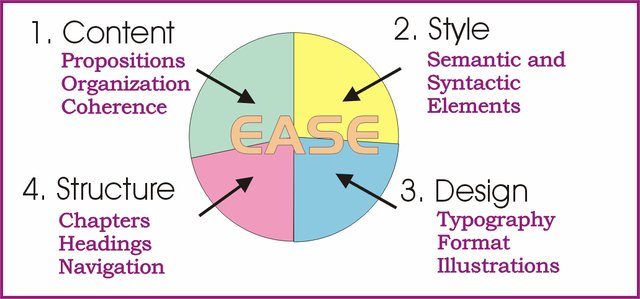
\includegraphics[width=9cm]{img/text-simplification-reading-ease.png}
	\end{center}
	\caption{Afbeelding van \textcite{Dubay2004}}
\end{figure}


\subsubsection{Lexicale wijzigingen}

Het onderzoek van \textcite{RiveroContreras2021} laat zien dat vereenvoudigde teksten de leessnelheid en woordherkenning van kinderen met visuele dysfunctie significant kunnen verbeteren. Uit het experiment van \textcite{Rello2013a} blijkt dat frequent woordgebruik de ontcijfertijd bij mensen met dyslexie significant vermindert en dat bevraagden met dyslexie minder leesfouten maken bij teksten met een verminderde lexicale complexiteit, volgens \textcite{Gala2016}. Het experiment benadrukt ook de moeilijkheden van kinderen met dyslexie bij het lezen van woorden met meer dan zeven karakters en onregelmatige en infrequente lettergreepcombinaties.

\begin{figure}
	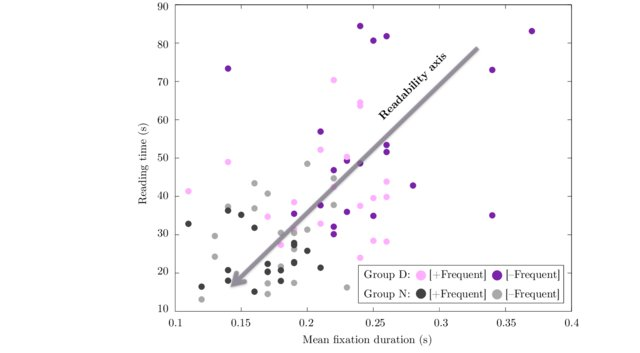
\includegraphics[width=\linewidth]{img/readability-mean-fixation-duration.png}
	\caption{Afbeelding van \textcite{Rello2013a}. Volgens de richting van de pijl wordt de ideale situatie benaderd, gekenmerkt door doelwaarden. Deze waarden worden bereikt door mensen zonder dyslexie onder optimale omstandigheden. Het gebruik van vaak voorkomende woorden vermindert de decodeertijd en verbetert de leesbaarheid voor mensen met dyslexie.}
\end{figure}

\subsubsection{Grammatische wijzigingen}

Onderzoek rond de effecten op syntactische vereenvoudiging bij kinderen en scholieren met dyslexie zijn in schaarse hoeveelheid. Het aanpassen causale structuren bij kinderen en jongeren met een lage leesgraad had een significant effect op het leestempo en de foutenmarge van de bevraagden uit het experiment van \textcite{Linderholm2000}. Bij de revisies werden coherentieonderbrekingen werden hersteld door extra uitleg te voorzien, alsook door tekstgebeurtenissen in een temporele of tijdsafhankelijke volgorde te plaatsen. Zowel vaardige als minder vaardige lezers hadden baat bij de revisies. Verbale parafrasering heeft geen significant effect op lezers met dyslexie volgens \textcite{Rello2013c}. De bevraagden waren 13 tot en met 37 jaar oud met een gemiddelde leeftijd van 21 jaar. Het tekstformaat bleef ongewijzigd, maar lettertypes werden wel aangepast. 

\subsubsection{Formaat- en structurele wijzigingen}
Geassisteerd samenvatten bevoordeelt de leesbaarheid van een scholier met dyslexie volgens het experiment van \textcite{Nandhini2013}. De geassisteerde samenvatting is gebaseerd op onaangepaste zinnen afkomstig uit de oorspronkelijke tekst. Het ontwerp bij dit experiment haalt de belangrijkste zinnen onaangepast uit de oorspronkelijke tekst, herorganiseerd deze volgens de structuur van de oorspronkelijke tekst en presenteert deze aan de lezer. Al werd de logische structuur van de gepresenteerde zinnen in vraag gesteld, de leesbaarheid van de bevraagden was significant beter dan bij de oorspronkelijke tekst zonder een nadelig effect op de verstaanbaarheid van de bevraagden.

\subsubsection{Visuele presentatie}
Experimenten tonen aan dat scholieren met dyslexie gevoeliger zijn voor veranderingen in visuele parameters zoals lettertype, karakterafstand, tekst- en achtergrondkleur en grijswaarden. Aanbevolen kleurencombinaties zijn een lichtgrijze achtergrond met zwart lettertype op een gele achtergrond, of zachtgele, -groene of lichtblauwe achtergrondkleuren \autocite{Rello2015, Bezem2016, Rello2017}. Minimalistische ontwerpen met pictogrammen en afbeeldingen hebben een positief effect op de leesbaarheid van tekst. Lettergrootte groter dan 14pt en een sans-serif, \textit{monospaced} of \textit{roman} lettertype vergroten de leessnelheid. Het gebruik van lettertypes zoals OpenDys heeft geen effect op lezers met of zonder dyslexie, terwijl cursieve lettertypes worden afgeraden \autocite{Rello2013b, Rello2015}.

\begin{figure}[H]
	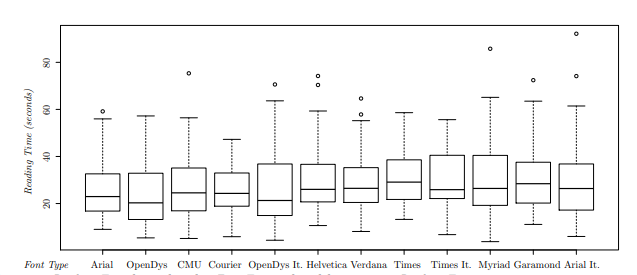
\includegraphics{img/fonts-readability.png}
	\caption{Afbeelding uit \textcite{Rello2013b}. Verticaal wordt de gemiddelde mening van de bevraagden weergegeven. Horizontaal worden de lettertypes gerangschikt op gemiddelde leestijd van alle bevraagden. Dit onderzoek wijst uit dat Arial, CMU, Helvetica en Times de populaire keuzes zijn. Arial en CMU behoren hierbij tot de drie best scorende lettertypes rond gemiddeld leestempo.}
\end{figure}

\subsection{Conclusie}
Op basis van de literatuurstudie kan besloten worden dat het aanpassen van teksten een significant effect heeft op de leessnelheid en woordherkenning van jongeren met dyslexie. Het vereenvoudigen van de lexicon en het toepassen van frequente woorden zorgt voor een verminderde decodeertijd en verbetert de leesbaarheid van teksten. Bevraagden met dyslexie hebben minder moeite met het lezen van teksten met verminderde lexicale complexiteit en geassisteerd samenvatten van teksten verbetert de leesbaarheid. Ook het aanpassen van de tekstweergave, zoals het gebruik van zachtgele, -groene of lichtblauwe achtergrondkleuren, kan de leeservaring van scholieren met dyslexie verbeteren. Het onderzoek rond de effecten op syntactische vereenvoudiging bij kinderen en jongeren met dyslexie is echter beperkt.

\section{Wetenschappelijke artikelen}
Wetenschappelijke artikelen volgen een uniform IMRAD-formaat en worden gebruikt als leermiddel voor jongeren in het middelbaar en hoger onderwijs. Het lezen van deze artikelen brengt uitdagingen met zich mee vanwege de verschillen in syntax en woordenschat. Docenten kunnen dit aanpakken in de derde graad van het middelbaar onderwijs door te benadrukken wat de specifieke kenmerken van wetenschappelijke artikelen zijn. In deze sectie wordt de volgende onderzoeksvraag beantwoordt: "Wat zijn de specifieke kenmerken van wetenschappelijke artikelen?"

\subsection{Trends rond wetenschappelijke artikelen}
De leesgraad van wetenschappelijke teksten volgt al sinds de tweede helft van de twintigste eeuw een stijgende trend \autocite{Hayes1992}. Meerdere onderzoeken in de voorbije tien jaar besluiten dat de complexe woordenschat en zinsbouw deze wetenschappelijke artikelen ontoegankelijk maakt voor doelgroepen naast onderzoekers \autocite{Ball2017, PlavenSigray2017, Jones2019}. \textcite{PlavenSigray2017} onderzoekt de verschillende trends waarom wetenschappelijke artikelen alsmaar moeilijker te lezen worden. De relatie tussen de leesbaarheid van een abstract werd vergeleken met het jaar waarin het wetenschappelijk artikel werd gepubliceerd. De \textit{Flesch-Reading-Ease} of FRE score werd gebruikt om de leesgraad van een wetenschappelijk artikel te beoordelen. Om te bevestigen dat de relatie tussen de complexiteit van een abstract overeenstemt met die van de volledige tekstinhoud, werden er vergelijkingen gemaakt met zes verschillende wetenschappelijke journalen. De overeenkomst tussen de leesgraad van het abstract en de overige tekstinhoud in een wetenschappelijk artikel werd eerder bevestigd door \textcite{Dronberger1975}. Dat onderzoek benadrukte dat een abstract complexer werd geschreven, vergeleken met de rest van een wetenschappelijk artikel.

\begin{figure}[H]
	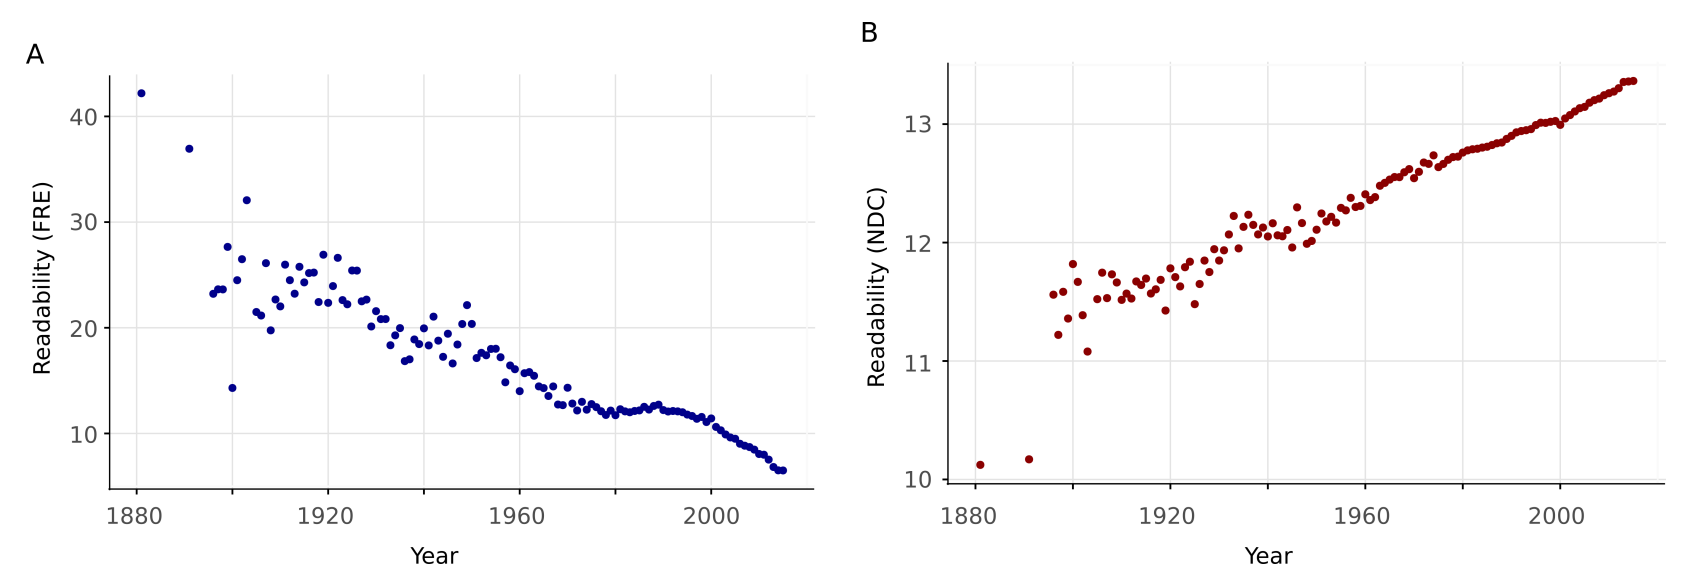
\includegraphics[width=\linewidth]{img/fre-ndc.png}
	\caption{Afbeelding uit \textcite{PlavenSigray2017}. Links wordt de evolutie per FRE-score getoond. Hoe hoger de score, hoe hoger de gemiddelde complexiteit van een tekst. Rechts wordt de evolutie volgens de NDC-score getoond. Hoe hoger de score, hoe lager de gemiddelde complexiteit van een tekst. Het onderzoek schat dat nu een kwart van alle wetenschappelijke artikelen gebruik maken van Engels op het niveau van een masterstudent, ofwel een FRE onder nul.}
\end{figure}

De hoge leesgraad van wetenschappelijke artikelen beperkt volgens \textcite{PlavenSigray2017} twee aspecten: de toegankelijkheid en de herproduceerbaarheid.

\subsubsection{Toegankelijkheid}
Het belang van toegankelijke wetenschappelijke inhoud wordt ook benadrukt door \textcite{Snow2010}, die stelt dat wetenschappelijke kennis een belangrijke rol speelt in het dagelijks leven en dat het daarom van groot belang is om wetenschappelijke informatie begrijpelijk te maken voor het bredere publiek. Dit kan de wetenschappelijke gemeenschap helpen om meer vertrouwen en steun te krijgen vanuit de samenleving en kan bijdragen aan het oplossen van problemen die voortkomen uit wetenschappelijke kwesties, zoals klimaatverandering. Om dit te bereiken, pleiten zowel \textcite{Ennals2010} als \textcite{Snow2010} voor het gebruik van eenvoudigere taal en duidelijkere zinsstructuren in wetenschappelijke communicatie. Door wetenschappelijke informatie toegankelijker te maken, kan de wetenschap beter bijdragen aan de maatschappij als geheel.

\subsubsection{Reproduceerbaarheid}
Wetenschappelijke artikelen kunnen zelfs voor vakexperten onbegrijpelijk zijn door complexe zinsstructuren en ontoegankelijke woordenschat. Om de begrijpbaarheid te vergroten, is het volgens onderzoekers als \textcite{Hartley1999} en \textcite{Snow2010} belangrijk om abstracten te herschrijven. Voor wetenschappers is het cruciaal dat hun onderzoeken reproduceerbaar zijn, wat betekent dat de inhoud van het wetenschappelijke artikel begrijpelijk moet zijn. Een lage leesgraad en duidelijke zinsbouw kunnen het aantal misopvattingen en verwarringen bij onderzoekers beperken. Experimenten van \textcite{Hubbard2017} tonen aan dat zowel de methodologie als de resultaten van wetenschappelijke artikelen een hoge leesgraad vereisen, wat het belang onderstreept van begrijpelijke wetenschappelijke taal.

\subsection{Woordenschat en vakjargon}
Wetenschappelijke artikelen maken gebruik van complexe processen, methoden en ideeën, verwoord met academische taal die zich onderscheidt van taal van een lagere leesgraad. Hoewel de kenmerken van academische taal variëren afhankelijk van de discipline, het onderwerp en de vorm, zijn er gemeenschappelijke kenmerken die wetenschappelijke taal onderscheiden \autocite{Ennals2010, Snow2010}. Volgens \textcite{PlavenSigray2017} dienen wetenschappelijke artikelen in eerste instantie als uitwisseling van kennis tussen vakexperten. Echter, de lengte van deze artikelen kan een nadelig effect hebben op de beschikbare uitleg van de terminologie. Daarom moet er in STEM-vakken of vakken waar deze wetenschappelijke artikelen aan bod komen, voldoende uitleg over de toegepaste grammatica en woordenschat worden voorzien tijdens de lessen, zoals benadrukt door \textcite{Snow2010}.

\begin{figure}[H]
	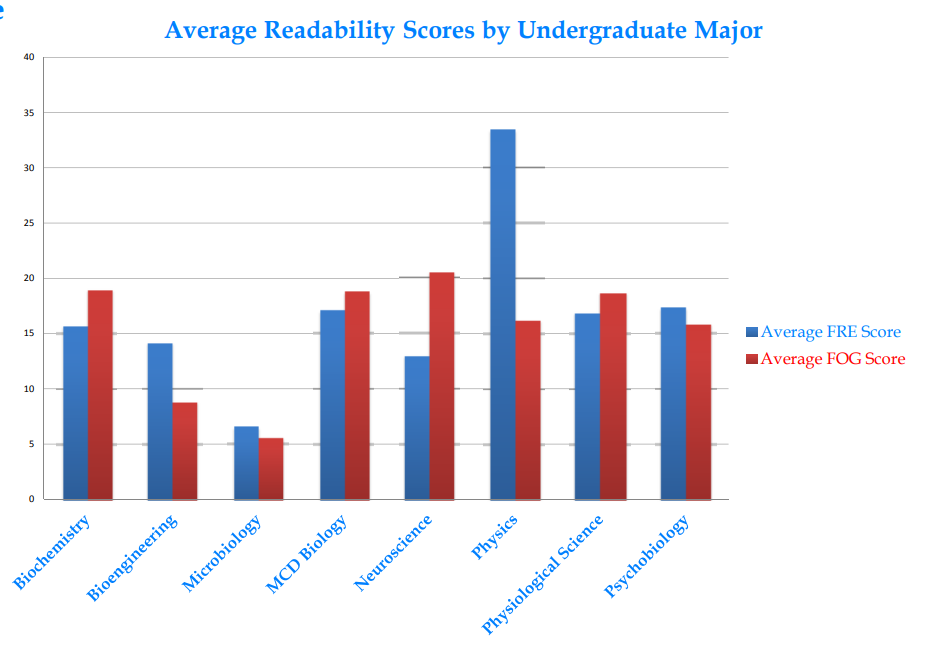
\includegraphics[width=5cm]{img/fre-fog-per-sector.png}
	\caption{Afbeelding van \textcite{Murdos2014} Volgens deze grafiek scoren de wetenschappelijke artikels rond fysica gemiddeld het best op de FRE-score. Al scoren de wetenschappelijke artikels rond microbiologie gemiddeld het zwakst op de FRE-score, ze scoren gemiddeld beter op de FOG-score.}
\end{figure}

\subsection{Aanpak voor het lezen van wetenschappelijke artikelen}
Als reactie op een satirisch artikel van \textcite{Ruben2016}, bracht \textcite{Pain2016} het onderwerp bij wetenschappers aan het licht om zo verschillende tactieken te verzamelen om wetenschappelijke artikelen te begrijpen. Sommige wetenschappers zoeken direct onbekende woorden op of raadplegen extra informatiebronnen, terwijl andere wetenschappers hoofdstukken overslaan. Het is belangrijk om een balans te vinden tussen het begrijpen van de inhoud en het efficiënt gebruiken van de tijd. Sommige wetenschappers geven toe dat ze het soms opgeven als het te moeilijk wordt of als de literatuur net niet relevant is voor hun onderzoek. \textcite{Pain2016} bouwt verder op deze adviezen en bouwt een stappenplan op hoe lezers wetenschappelijke artikelen kunnen aanpakken.

\begin{enumerate}
	\item Lees de samenvatting en conclusie om een idee te krijgen van het doel en de uitkomst van het onderzoek.
	\item De figuren en tabellen in het artikel zijn cruciaal omdat deze een snelle en duidelijke weergave geven van de belangrijkste bevindingen.
	\item Focus op de nodige informatie en ga vervolgens terug om de technische details te begrijpen.
	\item Let op de beperkingen en interpretatie van de resultaten. Controleer of de onderzoeksvraag en -methode adequaat zijn.
	\item Controleer of de referenties relevant zijn en zoek naar andere artikelen over hetzelfde onderwerp.
	\item Overweeg welke stukken prikkelend, nieuw en relevant zijn voor eigen onderzoeksvragen en hypotheses.
	\item Maak annotaties en schrijf tijdens het lezen, zodat de lezer actief betrokken is bij het lezen van het artikel.
\end{enumerate}

Wetenschappelijke artikelen vereisen een selectieve en kritische leesstijl. Onderzoekers geven aan dat ze bepaalde delen van een artikel prioriteren, zoals de abstract en de discussie, om te bepalen of het artikel de moeite waard is om te lezen. Sommige onderzoekers adviseren om de methodologie over te slaan en direct naar de resultaten te gaan, terwijl anderen juist de hypothese willen kennen voordat ze verder gaan. Het artikel wordt vervolgens meermaals gelezen, waarbij de lezer steeds dieper ingaat op de details. Kritisch lezen is hierbij van groot belang, waarbij de conclusies worden beoordeeld en de data voor zichzelf spreekt. Er is geen standaardaanpak, maar er worden tactieken aanbevolen zoals selectief en met een specifiek doel voor ogen lezen. Het doel van deze selectieve leesstijl is om de wetenschappelijke inhoud beter te begrijpen en te beoordelen op relevantie voor het eigen onderzoek \autocite{Hubbard2017}.

\subsection{Conclusie}

Het lezen van wetenschappelijke artikelen kan overweldigend zijn, vooral bij onbekende vakgebieden, lange artikelen en technisch vakjargon. Nieuwe versies van een wetenschappelijk artikel moeten meer doelgroepen toelaten om over voldoende achtergrondinformatie te beschikken. De gebruikte syntax, woordenschat en compact formaat sluiten aan bij de mogelijke struikelblokken voor ee scholier met dyslexie in de derde graad van het middelbaar onderwijs. 

\section{Tekstvereenvoudiging}
Vereenvoudigde teksten worden geschreven om leerlingen te ondersteunen bij het begrijpen van specifieke taalkenmerken, het beperken van de hoeveelheid nieuwe woordenschat en het beheersen van de complexiteit van de tekst. Deskundigen zijn van mening dat vereenvoudigde teksten nuttig zijn voor startende en gevorderde lezers \autocite{Louwerse2007}. Samenvattingen van teksten bieden een oplossing om een snel zicht te krijgen over (lange) documenten, of om de kerninhoud van een tekst die al gelezen is opnieuw te prikkelen \autocite{McCombes2022}. Vereenvoudigen kan handmatig door de docent gebeuren, maar recente technologische ontwikkelingen laten de automatisatie van dit proces toe met een gelijkwaardig eindresultaat. Deze sectie beantwoordt de volgende onderzoeksvraag: "Welke aanpakken zijn er voor geautomatiseerde tekstvereenvoudiging?". Aansluitend hierop wordt de volgende subvraag beantwoordt: "Hoe worden teksten handmatig vereenvoudigd voor scholieren met dyslexie?"

\subsection{Manuele tekstvereenvoudiging}

Wetenschappelijke artikelen moeten informatie begrijpelijk weergeven voor een breed publiek, waaronder de scholieren die deze artikelen voorgeschoteld krijgen. Teksten vereenvoudigen heeft volgens \textcite{Crossley2012} drie algemene doelen, namelijk het illustreren van een specifiek taalkenmerk, ongekende woordenschat voor een doelgroep aan te passen en de hoeveelheid gegeven informatie onder controle te houden. \textcite{Crossley2012} wijst op twee soorten van handmatige tekstvereenvoudiging. Intuïtieve tekstvereenvoudiging is een methode waar de auteur die de transformatie uitvoert, wordt beïnvloed door persoonlijke vermoedens over wat een tekst beter leesbaar maakt. Structurele vereenvoudiging daarentegen vervangt vermoedens door het gebruik van woordenlijsten en leesbaarheidsformules zoals Flesch Reading Ease (FRE), Gunning Fog (FOG), SMOG-Cro (SMOG) en de Coleman-Liau Index (CLI). Het onderzoek van \textcite{Crossley2012} wijst het bevorderend effect van de unieke aanpakken per docent uit. Iedere docent heeft een eigen intuïtie of afweging waarop teksten kunnen worden vereenvoudigd. Er is geen uniform formaat waarin een tekst kan worden vereenvoudigd. 

\subsubsection{Lengte en formaat}

Een samenvatting verkort de tekst door kernzinnen en trefwoorden te markeren of te parafraseren. Dit vereist meerdere lezingen van de tekst. Trefwoorden achterhalen gebeurt gelijkaardig en deze zijn regelmatig af te leiden uit de inhoudstafel en titels. Er zijn verschillende soorten samenvattingen: informatief vervangt de tekst, indicatief bevat links naar andere bronnen, en kritisch bevat de kerninhoud en een opiniestuk \autocite{Rijkhoff2022, Hahn2000}. Tekstvereenvoudiging vereenvoudigt complexe concepten en maakt de tekst begrijpelijker zonder betekenis of nauwkeurigheid te verliezen. Opsommingen benadrukken belangrijke punten en creëren structuur. Pragmatische vereenvoudiging zet metaforen, slang en idiomen om naar duidelijke taal. \textcite{Hahn2000} onderscheidt generieke en gebruikersgerichte samenvattingen, waarbij het belang van gebruikersgerichte samenvattingen wordt benadrukt door technologieën zoals full-text-search en gepersonaliseerde informatiefiltering. De opbouw van een gebruikersgerichte samenvatting omvat analyse van de brontekst, het aanduiden van de kernpunten en het samenvoegen tot één uitvoertekst. Een wetenschappelijke samenvatting moet volgens \textcite{Hollenkamp2020, McCombes2022} drie vragen beantwoorden: waarom werd het onderzoek verricht, wat werd er geëxperimenteerd en welke conclusies trekken de onderzoekers? Dit omvat de achtergrondinformatie, hypotheses, methoden, resultaten, implicaties, beperkingen en aanbevelingen. Alleen noodzakelijke kwalitatieve waarden moeten worden genoemd in de samenvatting. Vervolgens kan tekst naar een ander formaat worden omgezet, zoals \textit{post-itnotes}, tabelvorm of opsommingen om tekst begrijpelijker te maken \autocite{Rijkhoff2022}. 

% Een samenvatting verkort de lengte van een tekst. Kernzinnen en trefwoorden worden eerst handmatig in een tekst gemarkeerd en vervolgens op een nieuw blad geschreven. De kernzinnen worden achterhaald door enerzijds woord- en zoektermfrequentie en anderzijds door het stellen van algemene vragen over het artikel.  Voor deze twee methoden moet de persoon die een samenvatting maakt al vooraf de tekst meermaals gelezen hebben. Een alternatief op markeren is het parafraseren van de tekst. De geparafraseerde tekst is semantisch identiek, maar het neemt een andere syntax, structuur en woordenschat aan \autocite{Rijkhoff2022}. Volgens \textcite{Hahn2000} kan een samenvatting informatief, indicatief of kritisch zijn. Informatieve samenvattingen vervangen de oorspronkelijke tekst. Hoofd- en bijzaken zijn betrokken in de samengevatte tekst. Indicatieve samenvattingen behouden enkel een tekst met links die een lezer doorverwijzen naar andere bronnen. Kritische samenvattingen of \textit{reviews} bestaan uit de kerninhoud van de oorspronkelijke tekst en een opiniestuk over die specifieke kerninhoud. 

% Tekstvereenvoudiging omvat conceptuele of semantische vereenvoudiging door complexe concepten op te splitsen en duidelijke taal te gebruiken, pragmatische vereenvoudiging en het aanpassen van de alinea-indeling door middel van opsommingen. Het doel is om de tekst begrijpelijk te maken zonder betekenis of nauwkeurigheid te verliezen. Een opsomming of oplijsting benadrukt belangrijke punten en maakt een duidelijke structuur van een mogelijks complexe tekst \autocite{Siddharthan2014, Hale2022}. Pragmatische vereenvoudiging zet metaforen, \textit{short language} of \textit{slang} en idiomen om naar een letterlijke en duidelijke tekst \autocite{JavoureyDrevet2022}. Verder haalt \textcite{Hahn2000} ook het onderscheid tussen een generieke en een gebruikersgerichte samenvatting. Een generieke samenvatting staat niet stil bij speciale noden of interesses van de eindgebruiker in tegenstelling tot een gebruikersgerichte samenvatting waarbij er wel met sleutelwoorden of thema's in een tekst wordt rekening gehouden. \textcite{Hahn2000} haalt aan dat technologieën zoals \textit{full-text-search} en gepersonaliseerde informatiefiltering het belang van gebruikersgerichte samenvatting naar voor duwen. De opbouw van een gebruikersgerichte samenvatting omvat drie fasen volgens \textcite{Hahn2000}. Allereerst wordt de brontekst geanalyseerd. Daarna worden de kernpunten in een tekst aangeduid. Deze kernpunten kunnen verschillen per auteur. Ten slotte worden de punten samengevoegd tot één uitvoertekst.


\subsection{Natural Language Processing}

Tekstvereenvoudiging is het proces waarin het technisch leesniveau en/of woordgebruik van een geschreven tekst wordt verminderd. Het resultaat van deze fase is een tekst die korter en aangenamer is, zonder het verlies van de kerninhoud. Binnen machinaal leren (ML) is tekstvereenvoudiging een zijtak van natuurlijke taalverwerking. \autocite{Siddharthan2006} Volgens \autocite{Siddharthan2014} bestaat een complete en geautomatiseerde tekstvereenvoudiging uit vier verschillende vereenvoudigingen. \textit{Natural Language Processing} (NLP) of natuurlijke taalverwerking is een brede term die zich richt op het verwerken en analyseren van menselijke taal door computers \autocite{Eisenstein2019}. NLP omvat verschillende technieken, zoals tekstanalyse, taalherkenning en -generatie, spraakherkenning en -synthese, en semantische analyse. Computers zijn in staat om op een menselijke manier te communiceren en begrijpen wat er wordt gezegd. De volgende begrippen worden aangehaald in \textcite{Sohom2019, Eisenstein2019} en zijn fundamenteel voor de concepten die volgen.

\subsubsection{Tokenisatie}

% Tokenisatie splitst de stam of basisvorm van woorden in een tekst. Gebruikelijk zetten ontwikkelaars deze stap in om een woordenschat voor een taalmodel op te bouwen. Bij tokenisatie wordt er geen rekening gehouden met de betekenis achter ieder woord. Tokeniseren kan volgens  op woord-, karakter-, subwoord- en zinniveau. Karakterniveau heeft volgens  op zich weinig betekenis, alsook maakt deze vorm de inputlengte groter. Veelvoorkomende woorden worden hele woorden getokeniseerd, terwijl zeldzamere woorden opgesplitst worden in kleinere stukken die kunnen worden gebruikt. De rest van de woorden in de relevante dataset te creëren. Dit biedt een voordeel ten opzichte van word-level tokenisation omdat het een balans biedt tussen WLT en CLT .

Tokenisatie splitst tokens in een tekst en bouwt zo een woordenschat voor een taalmodel op. Dit kan volgens \textcite{Menzli2023} op woord-, karakter-, subwoord- en zinniveau gebeuren. Bij karakter-tokenisatie wordt de inputlengte groter en heeft daarmee volgens \textcite{Ribeiro2018} weinig betekenis. Zeldzame woorden worden opgesplitst in kleinere stukken om een woordenschat op te bouwen. Dit biedt voordelen ten opzichte van word-level tokenisatie \autocite{Iredale2022}.

\subsubsection{Lemmatiseren}

Lemmatiseren in NLP bouwt verder op \textit{stemming}, maar de betekenis van ieder woord wordt in acht genomen. Voor het lemmatiseren bestaan er Nederlandstalige modellen, waaronder JohnSnow\footnote{https://nlp.johnsnowlabs.com/2020/05/03/lemma\_nl.html}. Bij \textbf{omgekeerd lemmatiseren} wordt er een afgeleide achterhaald vanuit de stam. Voor zelfstandige naamwoorden, zoals 'hond', is dit enkelvoud of meervoud \autocite{Eisenstein2019}. Bij een \textbf{parsing}-fase wordt er een label aan ieder woord of zinsdeel toegekend. Voorbeelden van labels zijn zelfstandig naamwoord, bijwoord, werkwoord, bijzin of stopwoord. Het herkennen van zinsdelen wordt \textit{chunking} genoemd. Parsing heeft een dubbelzinnigheidsprobleem, want een 'plant' staat niet gelijk aan de vervoeging van werkwoord 'planten' \autocite{Eisenstein2019}.

% Sentimentanalyse is het achterhalen van de mening of gevoelens uit een tekst. de stemming of mening van een tekst te achterhalen op basis van het onderwerp. is een tak van Natural Language Understanding of NLU die de stemming, mening of gevoelens van de schrijver of spreker probeert te achterhalen ten opzichte van het onderwerp. % Dit kan lastig zijn omdat niet elke tekst een duidelijk positief of negatief sentiment heeft. 

\subsubsection{Sequence labeling en part-of-speech tagging}

Een machine moet de betekenis achter ieder token kunnen vatten. Hier komt \textit{sequence labeling} aan de pas volgens \textcite{Eisenstein2019}. Elk woord in een tekst wordt gekoppeld aan een \textit{Part-of-Speech} (PoS) of \textit{Named-Entity-Recognition} (NER) label. Deze NLP-fase achterhaalt de structuur van een tekst. PoS-tagging richt zich op grammaticale categorieën van woorden, terwijl NER-labeling instaat voor het herkennen van specifieke entiteiten in een tekst. Bij PoS-tagging worden de woorden in een zin geanalyseerd. Elk woord wordt gekoppeld aan een grammaticale categorie, zoals een zelfstandig naamwoord, werkwoord, bijvoeglijk naamwoord of bijwoord. \textit{PoS-tagging} helpt bij het achterhalen van de syntactische structuur van een zin. Deze taak komt van pas bij parsing en machinevertaling. \textit{PoS-tagging} wordt aanschouwelijk gemaakt op \ref{fig:pos}. Namen van personen, organisaties en locaties worden herkend en geclassificeerd met NER-labeling. Met NER-labeling wordt volgens \textcite{Jurafsky2014} specifieke informatie uit tekst gehaald, zoals het identificeren van de namen van personen, plaatsen of bedrijven die in nieuwsartikelen worden genoemd, of het extraheren van belangrijke data of getallen uit financiële rapporten. Dit wordt aanschouwelijk gemaakt \ref{fig:ner}. \textcite{Li2018} benoemt vier vormen voor NER-labeling: \textit{dictionary-based}, \textit{rule-based}, \textit{ML-based} en \textit{deep learning-based}. De eerste twee gebruiken vooraf gedefinieerde woordenboeken en regels, terwijl de laatste twee gebruik maken van statistische of neurale netwerken om te leren hoe entiteiten te herkennen. Elke vorm gebruikt verschillende kenmerken en representaties om entiteiten te modelleren. \textcite{Poel2008} onderzocht \textit{PoS-tagging} met een neuraal netwerk voor Nederlandstalige teksten. Het model behaalde een nauwkeurigheid van 97,88\% voor bekende woorden en 41,67\% voor onbekende woorden en gebruikte de Corpus Gesproken Nederlands (CGN) als trainingsdata.

\subsubsection{Word embeddings}

NLP-systemen gebruiken embeddings om woorden numeriek te representeren en tekst te verwerken. Traditionele word embeddings bouwen een woordenschat op zonder de betekenis ervan op te volgen, terwijl contextual word embeddings wel de context van een woord begrijpen. BERT is een meertalig LLM dat contextual word embeddings gebruikt en getraind is op 110 miljoen parameters uit 104 verschillende talen, waaronder Nederlands. Voor de Nederlandse taal zijn er twee varianten van BERT\footnote{https://github.com/google-research/bert}, namelijk RobBERT en BERTje, waarvan RobBERT als krachtiger wordt beschouwd. Om de beste vervanging van woorden te bepalen, gebruikt het model de Substitution Ranking (SR) stap om substituties op basis van relevantie te rangschikken. % TODO

% NLP-systemen en machines moeten woorden, grammatica en nuancering kunnen begrijpen. Embeddings transformeren woorden tot een numerieke representatie, waarop een machine deze representaties kan aanleren om nadien tekst te verwerken. Traditionele word embeddings bouwen een woordenschat op met unieke woorden. De betekenis achter ieder woord wordt niet opgevolgd. Voorbeelden van traditionele word embeddings zijn Word2Vec en Glove. Contextual word embeddings lossen dit probleem op en houden rekening met de context waarin een woord wordt gebruikt. ELMo en BERT zijn voorbeelden van een model voor contextuele embedding. Deze vorm houdt de semantiek bij van een woord in een bepaalde context en is noodzakelijk wanneer een machine polysemantische woorden in een tekst moet begrijpen. Contextuele word embeddings worden vergkregen uit transformer-gebaseerde modellen. Ze worden verkregen door een volledige zin door te geven aan een pre-trained model. BERT is een meertalig LLM, getraind op 110 miljoen parameters uit 104 verschillende talen\footnote{https://github.com/google-research/bert/blob/master/multilingual.md#list-of-languages}, waaronder Nederlands. Dit taalmodel kent alternatieven die verderbouwen op het oorspronkelijke BERT-model. Voor de Nederlandse taal zijn er twee, namelijk RobBERT en BERTje. Volgens (..) is RobBERT de krachtigste van de twee modellen, waar BERTje compacter is. Vervolgens bepaalt de \textit{Substitution Ranking} of SR-stap welke vervanging de beste is uit een set van kandidaten. SR gebeurt door gegenereerde substituties op basis van relevantie te rangschikken.

\begin{figure}[H]
	\begin{center}
		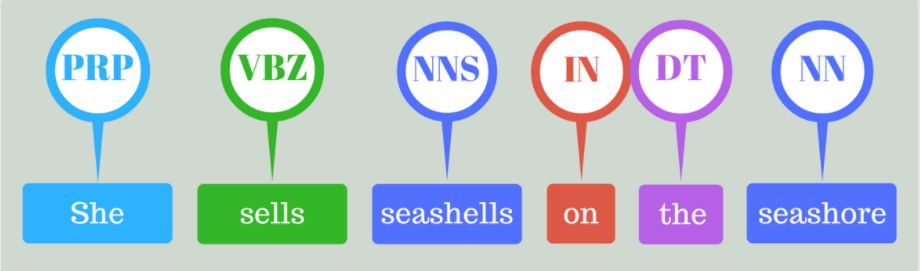
\includegraphics[width=10cm]{img/poslabeling.png}
	\end{center}
	\caption{Voorbeeld van PoS-labeling op de Engelstalige zin "She sells seashells on the seashore". Afbeelding van \textcite{Bilisci2021} }
	\label{fig:pos}
\end{figure}

\subsection{Prompt engineering}
Large Language Models of LLM's zoals GPT-3, BERT en T5 genereren tekst en karakters op basis van de probabiliteit of waarschijnlijke uitkomst van een gegeven input. Deze modellen maken gebruik van een neuraal netwerk om patronen in de input te herkennen en deze patronen te gebruiken om voorspellingen te doen over de uitvoer \autocite{Liu2020}. Iedereen kan volgens \textcite{McFarland2023} een input of prompt schrijven. Deze tools zoals chatbots zijn ontworpen om zo intuïtief mogelijk te zijn voor een algemeen doelpubliek. Prompt engineering is een steeds belangrijkere vaardigheid die nodig is om effectief te communiceren met LLM’s, zoals ChatGPT \autocite{Harwell2023}.

\begin{figure}
	\begin{center}
			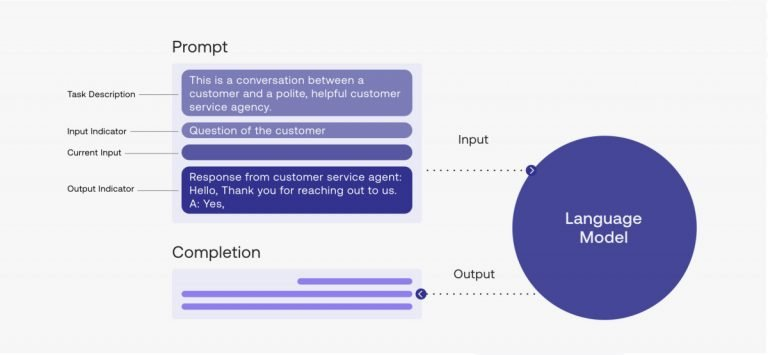
\includegraphics[width=8cm]{img/prompt-engineering-medium.png}
	\end{center}
	\caption{Afbeelding uit \textcite{McFarland2023}. Een illustratie over de werking en begeleiding van prompt engineering bij een taalmodel. }
\end{figure}

Deze prompts kunnen volgens \textcite{Liu2020} gebruikt worden om werk te produceren dat is aangepast aan het doel. Een concrete en geoptimaliseerde prompt omvat een concrete scope, duidelijke vraagstelling, specifieke sleutelwoorden, de context en ten slotte gepersonaliseerde keuzes \autocite{McFarland2023}. Bij een zoekopdracht moeten voldoende parameters in de prompt worden opgenomen. Zo niet zal het model te algemeen blijven en mogelijks afwijken van de intentie van de gebruiker. Effectieve AI prompt engineering leidt tot hoogwaardige trainingsgegevens die het AI-model in staat stellen om nauwkeurige voorspellingen en beslissingen te maken \autocite{Liu2020}. 

\subsubsection{Prompt patterns}

Prompt patterns is samen met prompt engineering naar boven gekomen en is vergelijkbaar met software patterns. Deze patronen zijn herbruikbare oplossingen voor veelvoorkomende problemen in een bepaalde context, waaronder vooral de interactie bij het werken met LLM's. \textcite{White2023} benoemt vier \textit{prompt patterns}:

\begin{itemize}
\item	Intent-prompts waarbij een LLM een instructie krijgt met een specfiek verwacht antwoord.
\item	Restriction-prompts die het antwoord van een LLM inperkt. Deze pattern is noodzakelijk om een LLM binnen de lijnen te houden.
\item 	Contextualization-prompts verzekeren dat de output van een LLM relevant is. Een context wordt aan de LLM meegegeven.
\item	Expansion/reduction-prompts genereren een beknopte output met voldoende details. 
\end{itemize}

\section{De verschillende soorten tekstvereenvoudiging}

Tekstvereenvoudiging bestaat volgens \textcite{Siddharthan2014} uit vier soorten transformaties: lexicale, syntactische en semantische vereenvoudiging en samenvatten.

\begin{figure}[H]
	\begin{center}
			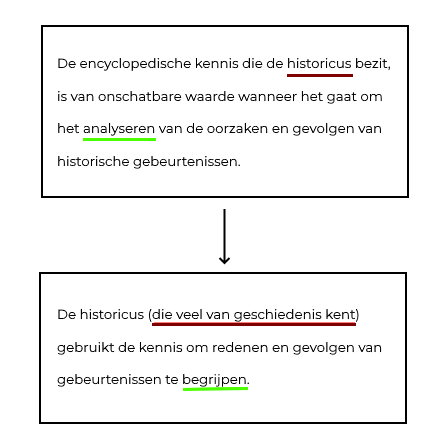
\includegraphics[width=5cm]{img/voorbeeld-manuele-vereenvoudiging.png}
	\end{center}
	\caption{Voorbeeld van tekstvereenvoudiging. Oorspronkelijke tekst uit Historia 5 bron toe te voegen}
\end{figure}

\subsection{Lexicale vereenvoudiging}

Bij \textit{lexical simplification} (LS) of lexicale vereenvoudiging worden complexe woorden vervangen door eenvoudigere synoniemen. Bijvoorbeeld, het woord 'adhesief' wordt vervangen door 'klevend'. \textcite{Kandula2010} haalt twee manieren aan om lexicale vereenvoudiging mogelijk te maken, namelijk het vervangen door een synoniem en het aanmaken of genereren van extra uitleg. De zinsstructuur verandert niet en er is garantie dat de kerninhoud en benadrukking in een tekst identiek blijft. Het doel van lexicale vereenvoudiging is om de moeilijkheidsgraad van de woordenschat in een zin of tekst te verlagen. 

\subsubsection{Complex Word Identification}

\textit{Complex word identification} (CWI) is een gesuperviseerde NLP-taak. In een pipeline voor lexicale tekstvereenvoudiging is CWI de eerste stap. Moeilijke woorden of \textit{multi-word expressions} (MWE) in een tekst worden achterhaald  \autocite{Shardlow2013, Gooding2019}. Na CWI kan LS gebruikt worden om deze woorden te vervangen door eenvoudigere synoniemen of om verdere elaboratie te voorzien met behulp van voorbeelden of definities \autocite{Zeng2005, Kandula2010}. CWI is volgens \textcite{Shardlow2013} een cruciale stap, want een lage \textit{recall} van dit component zal een uitvoertekst geven waar moeilijke woorden niet worden vereenvoudigd. Het model zal moeilijke woorden laten staan.

\subsubsection{Substitutiegeneratie en ranking}
Substitutiegeneratie wordt gedaan door synoniemen te zoeken voor een doelwoord in lexicale databanken zoals WordNet, BERT, context2vec, nPIC of OOC. 
\begin{figure}[H]
	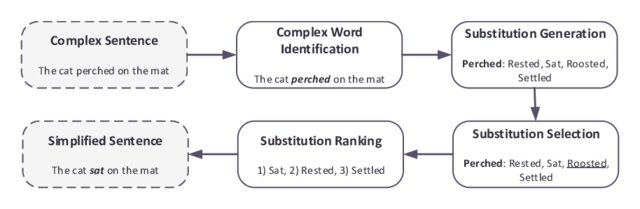
\includegraphics{img/lexical-simplification-pipeline.png}
	\caption{Afbeelding van \textcite{Althunayyan2021}. Deze pipeline wordt in meerdere onderzoeken rond lexicale vereenvoudiging toegepast, zoals \textcite{Paetzold2016, Bingel2018, Bulte2018}}
\end{figure}

\subsection{Syntactische vereenvoudiging}
Syntactische vereenvoudiging vermindert de complexiteit van een tekst door de grammatica en zinsstructuur aan te passen. Dit kan door het combineren van twee zinnen tot één eenvoudigere zin of door de syntax te vereenvoudigen. Deze transformaties verbeteren de toegankelijkheid van de tekst zonder de inhoud te verliezen. \textcite{Kandula2010} ontwikkelden een model om medische informatie te vereenvoudigen. Dit model omvat drie modules, die zinnen met meer dan tien woorden vereenvoudigen en eventueel vervangen door kortere zinnen. De architectuur omvat een PoS Tagger, een Grammar Simplifier en een Output Validator.

\begin{itemize}
	\item Voor de \textit{PoS Tagger}-fase gebruikten \textcite{Kandula2010} beschikbare functies uit het open-source pakket OpenNLP\footnote{https://opennlp.apache.org/}.
	\item De \textit{Grammar Simplifier} module splitst de lange zin in twee of meer kortere zinnen door POS-patronen te identificeren en een set transformatieregels toe te passen.
	\item De \textit{Output Validator} module controleert de output van de Grammar Simplifier op grammatica en leesbaarheid.
\end{itemize}  

\subsection{Tekstvereenvoudiging automatiseren}
Geautomatiseerde tekstvereenvoudiging is geen nieuw concept. Volgens onderzoeken van \textcite{Canning2000, Siddharthan2006} waren de eerste aanpakken op geautomatiseerde tekstvereenvoudiging gebouwd op rule-based modellen. Deze modellen bewerken de syntax door zinnen te splitsen, te verwijderen of de volgorde van de zinnen in een tekst aan te passen. Lexicale vereenvoudiging kwam hier niet aan de pas. Enkel bij recentere onderzoeken van \textcite{Coster2011, Bulte2018} werd het duidelijk hoe lexicale en syntactische vereenvoudiging gecombineerd kon worden.

\section{Samenvatten}

Lexicale, conceptuele en/of syntactische vereenvoudiging van teksten leidt niet altijd tot een kortere tekst. Technologieën zoals full-text-search en gepersonaliseerde informatiefiltering benadrukken het belang van gebruikersgerichte samenvatting. De architectuur van een samenvattingssysteem omvat drie fases: analyse van de brontekst, identificatie van kernpunten en het samenvoegen van de punten tot één uitvoertekst. Teksten machinaal samenvatten is geen nieuw concept en kan op twee manieren gebeuren: extraherend en abstraherend \autocite{Hahn2000, Dubay2004}.

% Teksten vereenvoudigen met lexicale, conceptuele en/of syntactische vereenvoudiging biedt geen garantie dat de tekstinhoud korter zal worden. Bij de drie soorten vereenvoudiging wordt er initieel enkel per zin gekeken. De vereenvoudiging houdt geen rekening met voorafgaande of opvolgende zinnen \autocite{Dubay2004}. Teksten machinaal samenvatten is geen nieuw concept. Het onderzoek van \textcite{Hahn2000} onderzoekt hoe teksten automatisch samengevat kunnen worden. Dit onderzoek haalt onder meer twee aanpakken aan hoe een machine teksten kan samenvatten, namelijk extraherend en abstraherend. Daarnaast reikt \textcite{Hahn2000} drie manieren aan welke inhoud er zeker in de samengevatte versie moet op te merken zijn.

% Generiek en gebruikersgerichte samenvatting
% Verder haalt \textcite{Hahn2000} ook het onderscheid tussen een generieke en een gebruikersgerichte samenvatting. Een generieke samenvatting staat niet stil bij speciale noden of interesses van de eindgebruiker. Daarnaast houdt een gebruikersgerichte samenvatting wel rekening met sleutelwoorden of thema's in een tekst. \textcite{Hahn2000} haalt aan dat technologieën zoals \textit{full-text-search} en gepersonaliseerde informatiefiltering het belang van gebruikersgerichte samenvatting naar voor duwen. \textcite{Hahn2000} omschrijft de architectuur van een samenvattingssysteem aan de hand van drie fases. Allereerst wordt de brontekst geanalyseerd. Daarna worden de \textit{salient points} of kernpunten in een tekst aangeduid. Deze punten zijn zinnen of tokens. Ten slotte worden de punten samengevoegd tot één uitvoertekst. De nadruk is verschillend per samenvattingsmethode.

\subsection{Extraherend samenvatten}

Bij extraherende samenvatting worden de belangrijkste zinnen gemarkeerd en opnieuw neergeschreven, maar dit kan leiden tot onsamenhangende uitvoertekst. Om de kernzinnen te achterhalen, zijn zes kenmerken volgens \textcite{Khan2014} essentieel, namelijk woordfrequentie, de plaats van een zin in de tekst, de \textit{cue method}, titels, de lengte van de zin, de gelijkenissen tussen de zin en de rest van het document, \textit{proper nouns} woordgebruik en ten slotte de afstand tussen \textit{text units} waarin entiteiten voorkomen. \textcite{Verma2020} onderzocht verschillende manieren om een tekst extraherend samen te vatten, waaronder graafgebaseerd extraherend samenvatten, maximal marginal relevance en meta-heuristic-gebaseerd samenvatten.

% Bij deze vorm worden de belangrijkste zinnen gemarkeerd en vervolgens opnieuw neergeschreven.  Dit is het equivalent van handmatig zinnen markeren en vervolgens op een blanco papier neerschrijven. Het nadeel hiervan is dat de uitvoertekst niet samenhangend kan zijn na het samenvatten. Kernzinnen achterhalen gebeurt bij geautomatiseerde samenvatting met zes features volgens \textcite{Khan2014}, namelijk de woordfrequentie, de plaats van een zin in de tekst, de \textit{cue method} of een woord dat de kerngedachte van een paragraaf benadrukt, titels, de lengte van de zin, de gelijkenissen tussen de zin en de rest van het document, het gebruik van \textit{proper nouns} en ten slotte de afstand tussen \textit{text units} waarin entiteiten voorkomen. De uitvoertekst kan coherentie en de oorspronkelijke structuur ontbreken. Dit maakt de uitvoertekst minder aangenaam om te lezen. \textcite{Verma2020} onderzocht de verschillende manieren waarop een tekst extraherend kan worden samengevat. Zij halen drie grote componenten aan, namelijk:

\subsubsection{Graafgebaseerd extraherend samenvatten}

De graafgebaseerde techniek van extraherend samenvatten vertegenwoordigt een document als een graaf van zinnen en gebruikt algoritmen om de belangrijkste zinnen te bepalen en redundantie te vermijden \autocite{Parveen2015}. Dit kan volgens \textcite{Parveen2015} zowel voor lange wetenschappelijke artikelen als korte nieuwsartikelen goede resultaten opleveren, vooral als coherentie en positionele informatie worden opgenomen. Het compacte SqueezeBERT-model kan ook worden ingezet voor real-time samenvatting, als een interessant alternatief op het grotere BERT-model, met bijna de helft van de grootte en minimale afbreuk in prestaties. Beide methoden kunnen de prestaties van NLP-downstream taken verbeteren \autocite{AbdelSalam2022}.

% Graafgebaseerd extraherend samenvatten is een techniek die een document voorstelt als een graaf, waarbij de knopen zinnen en bogen de relatie tussen de zinnen representeren. Deze algoritmen achterhalen de kernzinnen in een tekst. Bijvoorbeeld kan het PageRank-algoritme, dat vaak wordt gebruikt voor het rangschikken van webpagina's in zoekmachines, worden gebruikt om de zinnen in de grafiek te rangschikken op basis van hun belangrijkheid.

% \textcite{Parveen2015} raadt een graafgebaseerd systeem aan voor \textit{unsupervised learning}. Belangrijke zinnen worden met een lokaal minimum bepaald, alsook wordt redundantie vermeden. Deze methode kan significante resultaten opleveren bij het ophalen van kernzinnen uit zowel lange wetenschappelijke artikelen als korte nieuwsartikelen. Daarnaast vermeldt \textcite{Parveen2015} dat het systeem beter presteert wanneer coherentie wordt opgenomen en gecombineerd wordt met positionele informatie. % In toekomstig werk is \textcite{Parveen2015} van plan om meer taalkundige informatie in de entiteitsgrafiek op te nemen en beoordelingen van domeinexperts te verkrijgen om te zien of de redactiesamenvattingen als gouden samenvattingen kunnen worden gebruikt voor evaluatie.

% \textcite{AbdelSalam2022} voerden een vergelijkend onderzoek uit rond SqueezeBERT en BERT. De compacte architectuur van SqueezeBERT kan ingezet worden voor real-time samenvatting. Dit is volgens \textcite{AbdelSalam2022} een interessant alternatief op het BERT-model. In vergelijking heeft de voorgestelde SqueezeBERT slechts ongeveer 62 miljoen parameters, terwijl het prestatieniveau nog steeds boven de 90\% van het BERT-baseline model blijft. De evaluatie gebeurde aan de hand van de ROUGE-score. De onderzoekers besluiten dat SqueezeBERT een goed alternatief is, vooral door het trainen met bijna de helft van de grootte van het oorspronkelijke model en minimale afbreuk in de prestaties bij het samenvatten. Daarnaast kan het gebruik van efficiënte netwerken, zoals \textit{grouped convolutional layers}, de NLP-downstream taken verbeteren. 

% \textcite{AbdelSalam2022} haalt verder aan dat er potentie is voor een productieversie van een SqueezeBERT-samenvatter, die minder parameters heeft dan DistilBERT met ongeveer 20\% en dezelfde ROUGE-1 score behoudt, terwijl het iets hogere ROUGE-2 en ROUGE-L scores behaalt. Hoewel de SqueezeBERT en DistilBERT iets lagere scores produceren in vergelijking met het BERT-baseline model, heeft SqueezeBERT als voordeel dat het minder trainingstijd en minder parameters heeft dan het baseline model met ~48,44\%. 

\subsubsection{Maximal Marginal Relevance}

Traditionele samenvattingssystemen zijn gebaseerd op de architectuur van \textcite{Carbonell1998}, die gebruik maakt van de maximaal marginale relevantiescore (MMR) om de relevantie en diversiteit van gemarkeerde zinnen te bepalen. MMR zorgt ervoor dat de geselecteerde zinnen niet te veel overlappen in inhoud en relevantie. Onderzoekers hebben voorgesteld om het gulzige zoekalgoritme van MMR te vervangen door een globaal optimale formulering, wat een betere samenvatting oplevert, maar wel meer rekenkracht en tijd vereist. Evaluaties van deze methode tonen echter significant betere resultaten \textcite{McDonald2007, Lin2010}.

% Traditionele extraherende samenvattingssystemen bouwen verder op de door \textcite{Carbonell1998} ontworpen architectuur. Deze architectuur gebruikt een maximaal marginale relevantiescore of MMR. Deze architectuur houdt rekening met de diversiteit en de relevantie van de gemarkeerde zinnen. De relevantie van een zin in een tekst wordt bepaald door de mate waarin het taalmodel de belangrijkste informatie overbrengt van de tekst waarvan het afkomstig is. Om diversiteit aan tekstinhoud te waarborgen, wordt er gekeken naar de mate waarin de geselecteerde zinnen verschillen van de eerder geselecteerde zinnen in de samenvatting. Als een zin relevant is maar qua inhoud te veel overlapt met de eerder geselecteerde zinnen, dan heeft deze minder kans om in de geëxtraheerde samenvatting opgenomen te worden. Deze score kan doorgaans berekend worden met KeyBERT\footnote{https://maartengr.github.io/KeyBERT/api/mmr.html}.

% Extraherend samenvatten met de MMR-methode is de methode bij uitstek voor ML-toepassingen. Onderzoekers bouwen verder op de architectuur die beschreven staat in \textcite{Carbonell1998}. In \textcite{McDonald2007} stelt de onderzoeker voor om het gulzige zoekalgoritme van MMR te vervangen door een globaal optimale formulering, waarbij het MMR-framework wordt uitgedrukt als een knapzakprobleem of NP-volledig probleem. Daarmee wordt er gewezen naar een \textit{integer linear programming} (ILP) \textit{solver} die gebruikt kan worden om de wiskundige functie van MMR te maximaliseren. De MMR-methode hield voordien enkel rekening met relevantie en diversiteit, maar niet met de optimale combinatie van zinnen die in een samenvatting moet worden opgenomen. De aanpak van \textcite{McDonald2007} vereist echter meer rekenkracht en tijd dan de standaard MMR-methode, maar het experiment van \textcite{McDonald2007} haalde wel aan dat deze methode leidde tot significant betere resultaten. \textcite{Lin2010} evalueerde dit MMR-algoritme. Bij de evaluatie van deze architectuur benadrukte zij de significant betere resultaten. 

\subsubsection{Metaheuristiek-gebaseerd}

Metaheuristische samenvatting is een benadering die gebruik maakt van optimalisatie-algoritmen zoals genetische algoritmen, simulated annealing en zwermoptimalisatie om de belangrijkste zinnen in een tekst te vinden. Volgens \textcite{Premjith2015, Verma2020} zoeken deze algoritmen naar de beste combinatie van zinnen om de kerninformatie in de tekst te bevatten. De evaluatiefunctie kan verschillende criteria bevatten, zoals zinslengte, relevantie en verbanden, aldus \textcite{Rani2021}. Een beperking van deze methode is dat deze vaak vastloopt in een lokaal optimum en geen extremen of steilere hellingen op een zoekruimte aangeeft. Om de convergentie te versnellen, is het nodig om een optimalisatiestrategie te gebruiken die gebaseerd is op gradiënten.

% Metaheuristieke samenvatting maakt gebruik van metaheuristieke optimalisatie-algoritmen zoals genetische algoritmen, \textit{simulated annealing} of zwermoptimalisatie om de belangrijkste zinnen in een tekst te achterhalen. Deze algoritmen zoeken volgens  naar de beste combinatie van zinnen die de belangrijkste informatie in de tekst bevatten. De evaluatiefunctie in metaheuristieke samenvattingsalgoritmen kan gebaseerd zijn op verschillende criteria, zoals zinslengte, -relevantie en -verbanden.  benadrukt dat teksten samenvatten met een metaheuristieke methode regelmatig vastraakt in een lokaal optimum. Dit is een tekortkoming op andere methoden. Daarnaast wijst het onderzoek uit aan dat metaheuristieke methoden geen \textit{steepness} of extremen op een \textit{search space behaviour} aanduiden. Om de convergentie aanzienlijk te versnellen, moet er gebruik worden gemaakt van een optimalisatiestrategie gebaseerd op gradiënten. 

% gradienten: (een wiskundig concept dat de richting van de snelste toename aangeeft)
% convergentie: (het proces waarbij het algoritme naar de juiste oplossing toewerkt) -- Hierdoor wordt het algoritme efficiënter en sneller uitgevoerd.

\subsubsection{Experimenten over extraherend samenvatten}
% \subsubsection{title}

\textcite{McKeown1999} voerden experimenten uit op extraherende samenvattingen van nieuwsartikelen. De resultaten wijzen erop dat deze vorm vatbaar is op vooroordelen of \textit{bias} van de auteur. De zinnen worden genomen zoals ze zijn. \textcite{Hahn2000} bouwde verder op dit experiment. Zij voerden een experiment uit met een mix van \textit{knowledge-rich} en \textit{knowledge-poor} methoden, met significant positieve resultaten tot gevolg. De nadruk bij extraherend samenvatten ligt in het kiezen van de \textit{salient text units}. Deze punten zijn typisch in de vorm van zinnen. Er is nood aan een manier om de lexicale en statistische relevantie van een zin te kunnen aanduiden. Hiervoor haalt \textcite{Hahn2000} twee manieren aan:

\begin{itemize}
	\item Een lineair gewicht model. Iedere teksteenheid wordt gewogen op factoren zoals de \textit{location weight} en het aantal voorkomens.
	\item Een gewicht model op basis van de statistische opvallendheid van een eenheid. Zo wordt er rekening gehouden met de aanwezigheid van een woord in (sub)titels.
\end{itemize}

\textcite{Nallapati2017} wilden de nauwkeurigheid van deze modellen overbruggen. Dit doen ze met \textit{SummaRuNNer}\footnote{https://github.com/hpzhao/SummaRuNNer}, een oplossing voor het extraherend samenvatten van teksten met een neuraal netwerk. De toepassing werd opgebouwd met PyTorch in  en bestaat uit een combinatie van drie modellen: een recurrent neuraal netwerk, een convolutioneel recurrent neuraal netwerk en een \textit{hiërarchical attention network}.

\subsection{Abstraherend samenvatten}
Er zijn twee manieren om een tekst abstraherend samen te vatten: semantisch en structuurgebaseerd. De structuurgebaseerde benadering gebruikt regels om belangrijke informatie in de tekst te vinden en kan leiden tot samengevatte zinnen met lage linguïstische kwaliteit en grammaticale fouten. De semantisch-gebaseerde benadering gebruikt de betekenis van de tekst om korte en duidelijke samenvattingen te maken met minder redundante zinnen en betere linguïstische kwaliteit, hoewel een extra parsingfase nodig kan zijn. \textcite{Cao2022} heeft verder onderzoek gedaan naar deep learning methoden om automatisch abstraherende samenvattingen te genereren. Deep learning-modellen zoals RNN's, CNN's en Seq2Seq kunnen worden gebruikt voor abstraherend samenvatten door de betekenis van de tekst te begrijpen en belangrijke informatie over te brengen \autocite{Suleiman2020}. Het Pegasus-model, beschreven in \textcite{Zhang2020}, maakt gebruik van pre-trained modellen voor samenvatting met NLP en handelt gap-zinnen af, en is getraind en beoordeeld op verschillende soorten samenvattingstaken. LED of Longformer Encoder-Decoder is specifiek ontworpen om lange documenten te verwerken, waardoor het geschikt is voor het samenvatten van langere wetenschappelijke artikelen. 

% \textit{Deep learning} voor abstraherend samenvatten kan met verschillende modellen zoals RNN’s (terugkerende neurale netwerken), CNN’s (convolutionele neurale netwerken) en sequence-to-sequence (Seq2Seq) modellen. Deze modellen kunnen leren om samenvattingen te maken door de betekenis van de tekst te begrijpen en nieuwe tekst te maken die de belangrijkste informatie overbrengt \autocite{Suleiman2020}. Om een abstraherende samenvatting met deep learning op te bouwen bestaan er verschillende modellen. Het Pegasus-model beschreven in \textcite{Zhang2020} handelt \textit{gap-sentences} af met pre-trained models voor samenvatting met NLP.  Dit model werd getrained en beoordeeld op samenvattingstaken zoals emails, patenten, rekeningen en ook wetenschappelijke artikelen \autocite{Zhang2020}.

\subsection{Hybride samenvatten}

In het best denkbare geval wordt abstraherende en extraherende samenvatting gecombineerd volgens \textcite{Hsu2018, Huang2019}. Zo omvat een pipeline voor hybride samenvatting twee onderdelen: een \textit{content selection} fase waarin de kernzinnen met extraherende samenvatting worden opgehaald en \textit{paraphrasing}-fase waarbij de gemarkeerde kernzinnen abstraherend worden samengevat. 

\subsection{Evaluatie}

Samenvattingen van lange documenten handmatig beoordelen vergt tijd en voldoende planning van een mens \autocite{Nenkova2004}. Met behulp van een vooraf geschreven samenvatting als referentietekst is het mogelijk om een samenvatting automatisch te laten beoordelen. Samenvattingen beoordelen kan ook zonder referentietekst, al moeten verschillende factoren worden opgevolgd.

\subsubsection{Evaluatie met referentieteksten}

Bij het vergelijken van teksttransformaties worden vaak BLEU en ROUGE gebruikt, twee metrieken die de gelijkenis tussen machine-gegenereerde en referentieteksten meten gebaseerd op exacte \textit{token matches}. ROUGE volgens \textcite{Lin2004} is recall-gebaseerd en houdt geen rekening met synoniemen, maar er zijn ROUGE-modellen die dit wel doen. ROUGE-2 van \textcite{Ganesan2018} voorziet dictionaries van synoniemen, zodat er rekening wordt gehouden met synonieme zinnen. ROUGE-G van \textcite{ShafieiBavani2018} gebruikt graafalgoritmen om lexicale en semantische matching mogelijk te maken. BLEU is precision-gebaseerd is en een \textit{brevity penalty} introduceert om te korte teksten te voorkomen. Er zijn Python-bibliotheken beschikbaar voor zowel ROUGE\footnote{https://github.com/pltrdy/rouge} als BLEU\footnote{https://github.com/neural-dialogue-metrics/BLEU}.

\subsubsection{Evaluatie zonder referentieteksten}
Een samengevatte tekst beoordelen zonder een referentietekst vereist volgens \textcite{Steinberger2009} meer subjectiviteit en menselijke betrokkenheid dan met een referentietekst. Deze soort kan handmatig gebeuren, maar ook semi-automatisch. De type tekst, de lengte en de complexiteit van de oorspronkelijke tekst zijn factoren die in acht moeten worden genomen bij het beoordelen van de samengevatte tekst. Daar moet er worden gekeken naar het doelpubliek en het formaat. De tekst- en inhoudskwaliteit van de samengevatte tekst moet worden beoordeeld. De tekstkwaliteit is de grammaticale correctheid, niet-redundantie van zinnen en woordenschat en coherente structuur \autocite{McCombes2022}. De inhoudskwaliteit wijst op de informatie dat wordt opgenomen in de samengevatte tekst. Dit omvat de relevantie met de doelgroep bij kern- en bijzaken of misleidende informatie door een misinterpretatie van het systeem \autocite{McCombes2022}.


\subsection{Tekstvereenvoudigingstechnieken voor scholieren met dyslexie.}

In het onderzoek van \textcite{Bingel2018} wordt een systeem beschreven voor lexicale tekstvereenvoudiging, waarbij gebruik wordt gemaakt van een embeddings-gebaseerde aanpak voor substitution generation en een gesuperviseerd SR-model voor de selectie van synoniemen. Het systeem kan gepersonaliseerd worden op basis van gebruikersfeedback en maakt gebruik van een seed-dataset van complex-simple overeenkomsten. Het onderzoek van \textcite{DeBelder2010} richt zich op tekstvereenvoudiging voor kinderen van acht tot twaalf jaar en maakt gebruik van een methode voor lexicale en syntactische vereenvoudiging, terwijl \textcite{Bulte2018} een pipeline ontwikkelt om moeilijke woorden naar simpele synoniemen te vervangen, met behulp van een lexicale databank en LLM's.

% \textcite{Bingel2018} beschrijft een systeem voor dat gericht is op lexicale tekstvereenvoudiging en een embeddings-gebaseerde aanpak voor substitution generation. Tijdens de substitution selection maakt het systeem gebruik van een ongesuperviseerde boundary ranker om de synoniemen te filteren. De geselecteerde synoniemen worden vervolgens gerangschikt met behulp van een gesuperviseeerd SR-model. Daarnaast is het systeem in staat om het model te personaliseren op basis van gebruikersfeedback en maakt het gebruik van een seed-dataset van complex-simple overeenkomsten. Deze overeenkomsten houden rekening met de context van een woord in een zin en helpen bij de initiële vereenvoudiging van teksten. Alle gebruikersinformatie wordt met een PostgreSQL databank bijgehouden. Gebruikersinformatie wordt gekoppeld aan de demografische informatie informatie, om zo de ideale uitvoertekst te kunnen genereren. 

% Het onderzoek van \textcite{DeBelder2010} richt zich op tekstvereenvoudiging voor kinderen van acht tot twaalf jaar. Het onderzoek zet een methode op voor lexicale en syntactische vereenvoudiging. \textcite{Bulte2018} werkte het aspect rond lexicale vereenvoudiging verder uit. Het resultaat van dit onderzoek was een \textit{pipeline} ontworpen om moeilijke woordenschat naar simpele synoniemen te vervangen. Eerst ging de tekstinhoud door een \textit{preprocessing}-fase, samen met het uitvoeren van WSE. Daarna werd de moeilijkheidsgraad van ieder token overlopen. De moeilijkheidsgraad is gebaseerd op de frequentie in SONAR500\footnote{https://taalmaterialen.ivdnt.org/download/tstc-sonar-corpus/} een corpus met eenvoudige Nederlandstalige woorden, en ook de Wablieft-corpus, een archief van nieuwsartikelen in eenvoudig Nederlands. Synoniemen werden teruggevonden met Cornetto\footnote{https://github.com/emsrc/pycornetto}, een lexicale databank met Nederlandstalige woorden, samen met een \textit{reverse lemmatization} fase. Lexicale vereenvoudiging is ingewikkeld wanneer er geen eenvoudigere synoniemen zijn. In dat geval blijft een moeilijk woord voor wat het is. Voor deze toepassing maakten de onderzoekers gebruik van LLM's samen met Wikipedia annotaties. Deze annotaties bevestigden of de gegeven informatie correct is. De resultaten van deze toepassingen vallen in lijn met andere huidige toepassingen van hun soort. De onderzoekers benadrukken dat deze toepassing ook voor andere doelgroeppen met een lagere leesgraad kunnen dienen, zoals L2-lezers.

\begin{figure}[H]
	\begin{center}
			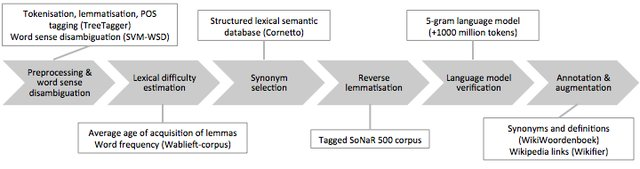
\includegraphics[width=9cm]{img/dutch-simplification-dyslexia-pipeline.png}
	\end{center}
	\caption{Afbeelding uit \textcite{Bulte2018}. Deze pipeline omvat de stappen die de toepassing aflegt. }
\end{figure}

\begin{figure}[H]
	\begin{center}
			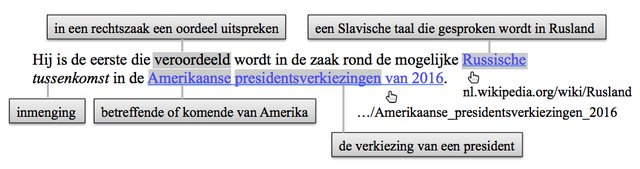
\includegraphics[width=9cm]{img/dutch-simplification-dyslexia-example.png}
	\end{center}
	\caption{Afbeelding uit \textcite{Bulte2018}. TODO}
\end{figure}


Al zijn er onderzoeken over lexicale, syntactische en semantische vereenvoudiging voor kinderen en scholieren met dyslexie, het aantal onderzoeken over samenvatten voor deze doelgroep is schaars. Zoals eerder aangehaald is er wel onderzoek gedaan naar de verschillende manieren om een tekst samen te vatten, maar er is geen toepassing of onderzoek dat dit concreet uitwerkt. 

\subsection{Conclusie}

Wetenschappelijke artikelen volgen een gelijke structuur. De inhoud in PDF- of afbeeldingvorm vergt voldoende cleaning-fasen. Het beoordelen van de samenvatting op basis van een referentietekst met de ROUGE-metriek wordt aangeraden, al kan deze beoordeling niet enkel machinaal gebeuren. Daarnaast is er input en bijsturing nodig van de mens omtrent een samenvatting op maat en de grammaticale, lexicale en semantische correctheid. Tools gericht op het lexicaal en adaptief vereenvoudigen van teksten voor kinderen en scholieren met dyslexie zijn reeds uitgewerkt. Methoden om menselijke en grammatisch correcte samenvatting op te bouwen zijn reeds beschikbaar. 

\section{Valkuilen en uitdagingen voor AI-ontwikkelaars bij tekstvereenvoudiging met AI}

AI en ML zijn volop in groei. NLP gebruikt AI en ML om menselijke taal te verwerken, terwijl NLU deze technologieën gebruikt om menselijke taal te begrijpen. Hoewel deze technologieën veelbelovend zijn, moeten AI-ontwikkelaars rekening houden met veelvoorkomende en genegligeerde uitdagingen en valkuilen \autocite{Sciforce2020, Roldos2020, Khurana2022}. Deze sectie beantwoordt de volgende onderzoeksvraag: "Met welke valkuilen bij taalverwerking met AI moeten ontwikkelaars rekening houden?"

\subsection{Uitdagingen voor softwarebedrijven}

NLP- en NLU-toepassingen behoren tot de duurste om te ontwikkelen, wat een obstakel kan vormen voor veel IT-professionals. Het gebrek aan NLP-expertise, de kwaliteit en kwantiteit van data, de integratie en deployment van modellen en de transparantie van modellen zijn allemaal factoren die bijdragen aan deze hoge kosten \autocite{IBM2022}. Software-ontwikkelaars verkiezen volgens  voor \textit{black-box} modellen bij de ontwikkeling en finetuning van een NLP-toepassing met AI. Al is het verschil qua nauwkeurigheid minimaal, de afweging wordt gemaakt bij de transparantie van het model. Na een transformatie wordt er niet aangegeven waarom specifieke transformaties werden uitgevoerd, bijvoorbeeld het vervangen van een woord door een eenvoudiger synoniem. White-box taalmodellen zijn er in schaarse hoeveelheden \autocite{Punardeep2020}. 

% Volgens het jaarlijks rapport van IBM behoren NLP en NLU-toepassingen tot de duurste soort om te ontwikkelen. Ongeveer 54\% van de bevraagde IT-professionals vond de bijhorende kosten een obstakel bij het starten van de ontwikkeling voor NLP-toepassingen. Professionals halen verschillende pijlers aan, waaronder de kwaliteit en kwantiteit van de data, het trainen van de data, het gebrek van NLP-experten, de integratie en deployment van de taalmodellen en ten slotte de transparantie van het model. Gespecialiseerde modellen zijn use-case afhankelijk wat ze niet voor iedere toepassing bruikbaar maakt. Als oplossing kunnen softwarebedrijven partnerships afsluiten, investeren in NLP-talent, klein starten en stelselmatig opschalen, cloud-gebaseerde oplossingen aanreiken of de transparantie van een model benadrukken in hun specifieke toepassing . Software-ontwikkelaars verkiezen volgens  voor \textit{black-box} modellen bij de ontwikkeling en finetuning van een NLP-toepassing met AI. Al is het verschil qua nauwkeurigheid minimaal, de afweging wordt gemaakt bij de transparantie van het model. Na een transformatie wordt er niet aangegeven waarom specifieke transformaties werden uitgevoerd, bijvoorbeeld het vervangen van een woord door een eenvoudiger synoniem. White-box modellen zijn er in schaarse hoeveelheden. 

\subsection{Ambiguïteit, synoniemen en homoniemen}

Homoniemen kunnen volgens \textcite{Roldos2020} problemen veroorzaken bij sequence labeling of het labelen van tokens in een doorlopende tekst. Bijvoorbeeld bij het woord ‘bank’ is het niet duidelijk voor de machine of het gaat over de geldinstelling of het meubel. Word Sense Disambiguation (WSD), PoS-tagging en contextual embeddings kunnen de betekenis van een woord achterhalen op basis van de context \autocite{Eisenstein2019, Liu2020}. Het gebruik van synoniemen en antoniemen in NLP-systemen kan verbeterd worden door het gebruik van candidate generation en synonym detection, en meertalige transformers zoals BERT bieden een oplossing voor het gebrek aan niet-Engelstalige toepassingen \autocite{Dandekar2016, Roldos2020}.

% Homoniemen kunnen echter roet in het eten gooien. Volgens heeft een machine moeite om de context van homoniemen te achterhalen. Bijvoorbeeld bij het woord ‘bank’ is het niet duidelijk voor de machine of het gaat over de geldinstelling of het meubel. \textit{Word Sense Disambiguation} of WSD achterhaalt de betekenis van een woord op basis van de context waarin een woord gebruikt wordt \autocite{Eisenstein2019}. Deze taak is nodig binnen NLP om rekening te houden met homoniemen. WSD implementeren kan dictionary-gebaseerd, gesuperviseerde, semi-gesuperviseerd of niet-gesuperviseerd. PoS-tagging kan dit probleem aanpakken volgens \textcite{Liu2020} als een oplossing op dit probleem, samen met het gebruik van contextual embeddings. Spacy biedt een sense2vec\footnote{https://github.com/explosion/sense2vec} aan.

% Bij het bouwen van NLP-systemen moeten zo veel mogelijke betekenissen en synoniemen van een woord worden opgenomen. Tekstanalysemodellen zijn niet foutloos, maar deze zullen synoniemen beter begrijpen als deze voldoende en relevante trainingsgegevens ontvangen \autocite{Roldos2020}. \textcite{Dandekar2016} reikt twee methoden aan: \textit{candidate generation} door gebruik te maken van word embeddings, historical user data of lexicale synoniemen. Dit kan ook gesuperviseerd met \textit{synonym detection}. Aanvullend kunnen antoniemen volgens \textcite{Dandekar2016} op eenzelfde manier worden achterhaald met NLP ML.

% Het onderzoek van \textcite{Sciforce2020} haalt aan dat het merendeel van NLP-toepassingen Engelstalige invoer gebruikt. Niet-Engelstalige toepassingen zijn zeldzaam. De opkomst van taalmodellen getrained op meertalige datasets en die meertalige transformers gebruiken, zoals BERT, biedt een oplossing op dit probleem en dempt de impact op ambiguïteit. \autocite{Roldos2020} % De taalmodel vertaalt eerst de oorspronkelijke tekst naar de gewenste taal, voordat de tekst wordt herwerkt. BERT maakt volgens  gebruik van meertalige transformers, wat de impact op verwarring kan dempen.

\subsection{Paternalisme en ethische overwegingen}

Tekstvereenvoudiging is bedoeld om gelijke kansen te bieden aan iedereen, maar ethische overwegingen en bewustzijn van de behoeften van de eindgebruiker zijn belangrijk bij het ontwikkelen van adaptieve tekstvereenvoudigingstoepassingen, zoals beschreven in onderzoeken van \textcite{Niemeijer2010, Xu2015, Gooding2022}. De eindgebruiker moet de keuze hebben om te kiezen welke delen van de tekst vereenvoudigd moeten worden, wat kan worden bereikt door synoniemen te kiezen of zinnen te markeren die moeilijk te begrijpen zijn.

% De doelstelling van ondersteunende toepassingen is om gelijke kansen te bieden aan iedere doelgroep. Tekstvereenvoudiging transformeert de oorspronkelijke tekst naar een tekst met een simpelere syntax, kortere zinnen, verminderde lexicale en semantische complexiteit en gereduceerd aantal zinnen. Volgens \textcite{Niemeijer2010} zijn de ethische overwegingen die samenhangen met tekstvereenvoudiging niet gemakkelijk te scheiden van de gebruikte technologie om het resultaat te bereiken. Het onderzoek van \textcite{Xu2015, Gooding2022} halen pijlers aan waarmee ontwikkelaars en softwarebedrijven rekening moeten houden bij de ontwikkeling van adaptieve en ondersteunende software voor tekstvereenvoudiging. Ontwikkelaars moeten zich meer bewust worden van de behoeften en verwachtingen van de eindgebruiker bij het ontwikkelen van een tekstvereenvoudigingstoepassing. Haar onderzoek benadrukt de paternalistische of afhankelijke aard van assisterende toepassingen. Tekstvereenvoudiging omvat vier transformaties, maar niet iedere transformatie is vereist voor iedere gebruiker. Een adaptieve tekstvereenvoudigingstoepassing moet de eindgebruiker een keuze aanbieden om aan te passen wat vereenvoudigd wordt, afhankelijk van specifieke behoeften. Om dit probleem op te lossen, is het belangrijk om de eindgebruiker, in dit geval scholieren met dyslexie in het derde graad middelbaar onderwijs, de keuze te geven. Zoals beschreven in \textcite{Gooding2022}, zijn er verschillende mogelijkheden. Bijvoorbeeld, de eindgebruiker moet de mogelijkheid hebben om te kiezen welke synoniemen de tekst lexicaal zullen aanpassen. Een alternatieve aanpak voor syntactische vereenvoudiging is om de scholier zelf zinnen te laten markeren die moeilijk te begrijpen zijn, zodat het systeem alleen de door de eindgebruiker aangegeven zinnen vereenvoudigt.

\subsection{Valkuilen bij prompt engineering}

% Iedereen is in staat om een conversatie met een chatbot op te bouwen. Het gebruik van de API voor een doelgericht en doordacht antwoord vergt echter planning bij de ontwikkelaar. \textcite{Miszczak2023} waarschuwt voor 'garbage-in garbage-out'. De kwaliteit van de input kan de kwaliteit van de output bepalen. \textcite{Jiang2023} benoemt de misopvatting bij de intentie van de gebruiker als de voornaamste uitdaging voor een taalmodel dat input vereist. Volgens Jiang kan dit te wijten zijn aan de gebruiker die een onvolledige prompt of een prompt met onvoldoende context op een concreet antwoord schrijft. Daarnaast kan een gebrek aan trainingsdata ook aan de oorzaak liggen van een onnauwkeurige uitvoertekst of bias in het taalmodel. Andere factoren die \textcite{Miszczak2023} aanhaalt, zijn de afwisselende probabiliteit van de outputtekst en de meegegeven parameters die het model beïnvloeden, zoals de temperature dat de creativiteit van het model beïnvloedt. Als oplossing kan de prompt als een conditionele expressie worden opgebouwd, zodat het taalmodel enkel met zekerheid een antwoord teruggeeft.

Het bouwen van een conversatie met een chatbot is voor iedereen mogelijk, maar het vereist doordachte input en planning bij de ontwikkelaar om kwalitatief hoogwaardige antwoorden te krijgen. Een onnauwkeurige prompt of gebrek aan trainingsdata kan leiden tot onjuiste output, terwijl het gebruik van conditionele expressies of finetunen van hyperparameters kan helpen de betrouwbaarheid van het antwoord te vergroten \autocite{Miszczak2023, Jiang2023}.

\subsection{Evaluatie en interpretatie}

ROUGE en BLEU zijn beperkt omdat ze geen rekening houden met semantiek, maar ROUGE-L, ROUGE-SU en METEOR wel \autocite{Raj2017, Tatman2019}. Menselijke evaluatie moet worden overwogen bij het onderzoeken van samenvattingsmethoden, en een mix van machinale en menselijke evaluatie is nodig volgens \textcite{Fabbri2020}. De onderzoekers stimuleren verder onderzoek naar nieuwe standaarden en best practices voor betrouwbare menselijke beoordeling op extraherende en abstraherende samenvattingen. De doelgroep waarvoor een tekst wordt samengevat, moeten nauw in het proces worden opgenomen \autocite{Iskender2021}.

\section{Beschikbare software voor tekstvereenvoudiging}

% inleiding voor welke software
Dyslexie is een veelvoorkomende aandoening die de lees- en schrijfvaardigheden van scholieren kan belemmeren. Om deze scholieren te ondersteunen, worden er verschillende softwareprogramma's en tools ontwikkeld. In dit hoofdstuk zal worden gekeken naar mogelijke nationale en internationale software die specifiek is ontworpen om scholieren met dyslexie te helpen bij het lezen van teksten. Er zal met name worden gekeken naar de beschikbare software in Vlaamse middelbare scholen, chatbots, zoals Bing AI en ChatGPT, en software die speciaal is ontwikkeld om dyslexie te ondersteunen bij het lezen. Deze sectie beantwoordt de volgende onderzoeksvraag: "Welke toepassingen, tools en modellen zijn er beschikbaar om Nederlandstalige geautomatiseerde tekstvereenvoudiging met AI mogelijk te maken?"

\subsection{Momenteel ingezet in het onderwijs}

In het middelbaar onderwijs wordt lees- en studieondersteuning voor scholieren met dyslexie enkel in de vorm van voorleessoftware voorzien \autocite{DeCraemer2018, OnderwijsVlaanderen2023}. \textcite{OnderwijsVlaanderen2023} leent licenties voor de volgende softwarepakketten uit SprintPlus, Kurzweil3000, Alinea Suite, IntoWords en TextAid. Naast luister- en schrijfopties kunnen scholieren deze toepassingen gebruiken om zinnen te markeren om deze zinnen vervolgens samen te vatten. Enkel de gemarkeerde zinnen worden betrokken in de samengevatte versie, dus de zinnen blijven lexicaal, syntactisch en semantisch identiek. Alle vermelde softwarepakketten bieden echter geen onafhankelijke samenvat- of vereenvoudigfunctie aan. \textcite{Tops2018} benadrukt de handige aspecten van deze software, maar deze software moet zo vroeg mogelijk in een schoolcarriére worden ingezet. Zo raken de scholieren snel vertrouwd met het gebruik, wat kan leiden tot een optimaal gebruik in verdere studies. Volgens \textcite{Tops2018} is het te laat om deze software pas in het hoger onderwijs te introduceren.

\subsection{Proof-of-concepts en online webapplicaties}

Online zijn er tools beschikbaar om teksten generiek samen te vatten. Resoomer, Paraphraser en Scholarcy zijn oorspronkelijk Engelstalige tools, met ondertussen de mogelijkheid om een abstraherende samenvatting te maken van Nederlandstalige teksten. De taalmodellen waar deze applicaties op werken, is niet gekend. Daarnaast zijn er ook geen API's beschikbaar om mee te werken. Gepersonaliseerde toepassingen zijn er in mindere mate. \textcite{Bingel2018} omschrijft een proof-of-concept voor een webtoepassing dat teksten vereenvoudigd, met oog op mensen met dyslexie. Deze software noemt nu Hero en bevindt zich in betafase.

Toepassingen om wetenschappelijke artikelen te vereenvoudigen zijn schaars, maar er zijn enkele gratis en betalende toepassingen beschikbaar. SciSpace\footnote{https://typeset.io/} is gratis. Scholarcy\footnote{https://www.scholarcy.com/?ref=theresanaiforthat} is betalend. 

\begin{figure}
	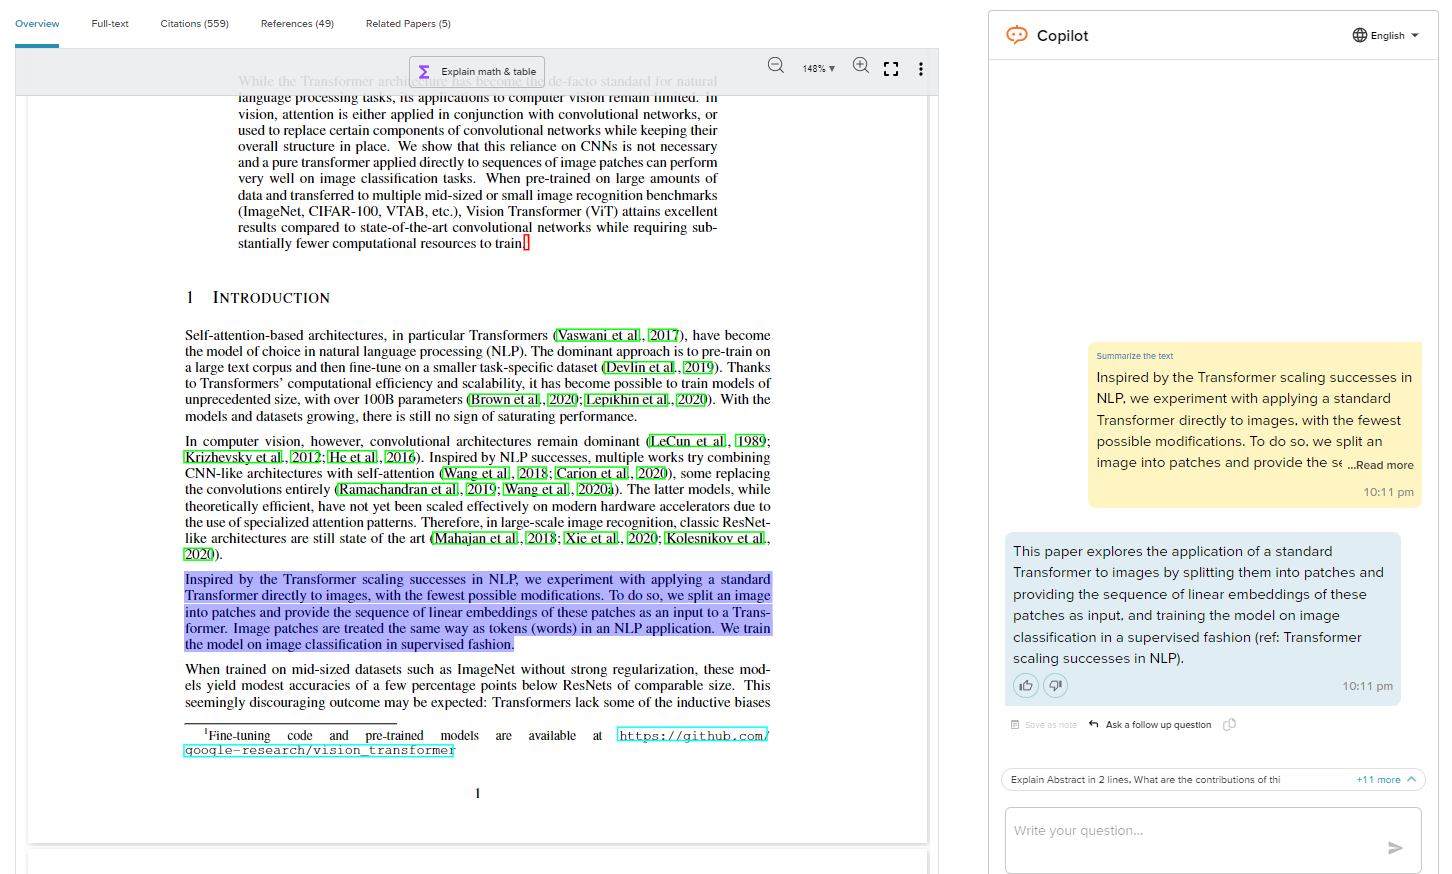
\includegraphics{img/typeset-example.png}
	\caption{Schermafbeelding van SciSpace}
\end{figure}

\section{GPT-3}
\textit{Generative Pretrained Transformer 3} of GPT-3 is een taalmodel ontworpen door OpenAI. Dit taalmodel gebruikt een tweestapsleerparadigma waarbij het eerst ongesuperviseerd wordt getraind met een taalmodelleringsdoel en daarna gesuperviseerd wordt gefinetuned. Over drie versies heen is het model aanzienlijk vergroot, van anderhalf miljard parameters bij GPT-2 naar 175 miljard parameters bij GPT-3. Het model is getraind op niet-gecategoriseerde data van het internet en gebruikt datasets waaronder Common Crawl, WebText2, Books1, Books2, and Wikipedia \autocite{Radford2019, Li2022}.

\begin{figure}[H]
	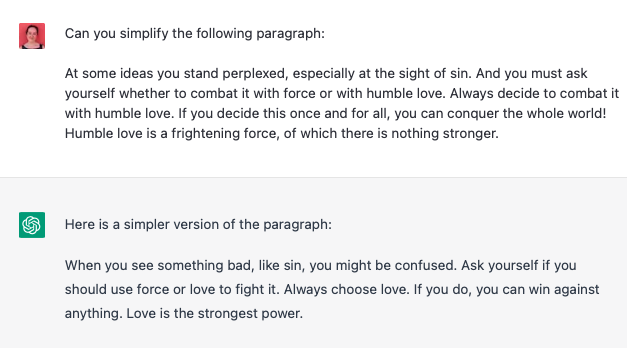
\includegraphics[width=10cm]{img/chatgpt-example-simplification-gooding.png}
	\caption{Afbeelding van Gooding 2022. De invoertekst is een paragraaf uit een niet-vermeld boek van de Russische schrijver Dostoevsky. Het resultaat van de meegegeven prompt is een transformatie dat iedere vorm van vooraf aangehaalde vereenvoudiging weergeeft. Lexicale, conceptuele en syntactische vereeenvoudiging worden op de invoertekst toegepast.}
\end{figure}

\begin{figure}[H]
	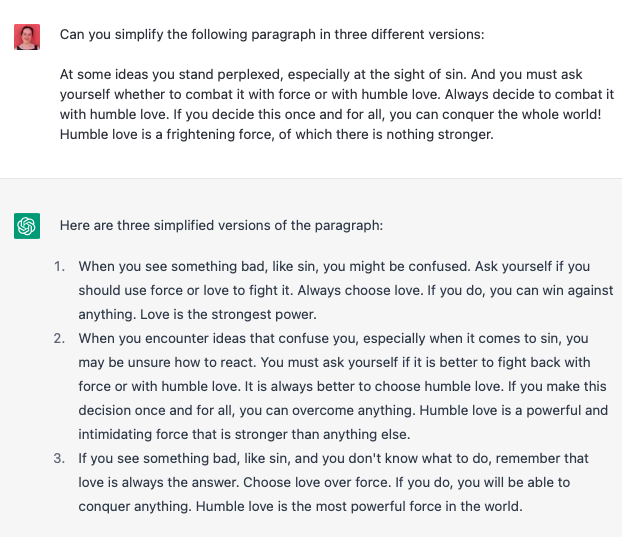
\includegraphics[width=10cm]{img/chatgpt-example-different-versions-gooding.png}
	\caption{Afbeelding van Gooding 2022. Gooding haalt verder aan dat modellen zoals ChatGPT op twee vlakken de leesbaarheid van een tekst kan bevorderen. Allereerst door het verlenen van verschillende mogelijke versies van een vereenvoudigingstaak.}
\end{figure}

\begin{figure}[H]
	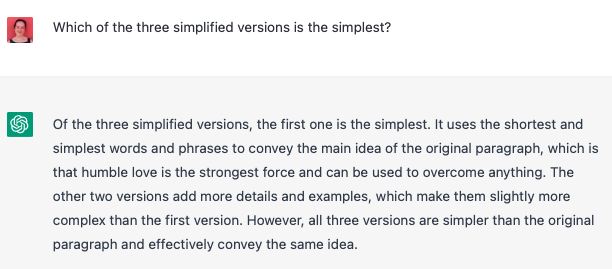
\includegraphics[width=10cm]{img/chatgpt-example-evaluation-gooding.png}
	\caption{Afbeelding van Gooding 2022.}
\end{figure}

\textcite{Lisowski2023} vergelijkt de twee OpenAI taalmodellen met een \textit{mixed-methods} onderzoek. Al blijken de twee heel gelijkaardig, het experiment benadrukt dat het ChatGPT-model gericht is op conversationele doeleinden met voorkeur als chatbot, terwijl GPT-3 een ML-model is bedoeld om met hoogstens één prompt te werken. De grootte van het GPT-3 model met 175 miljard parameters imposanter dan Chat-GPT. Daarnaast is de limiet bij het meest recente GPT-3 model is 4000 tokens. Verder haalt Lisowski aan dat de kwaliteit bij beide modellen sterk afhankelijk is van de invoer. De prompts moeten concreet genoeg zijn, om zo niet af te wijken van wat de gebruiker wilt \autocite{Lisowski2023}. Deze twee API's zijn nu vrij beschikbaar voor ontwikkelaars als betalende API \autocite{Brockman2023}.

\subsubsection{Beschikbare GPT-3 engines}

De documentatie van OpenAI\footnote{https://platform.openai.com/docs/} reikt vier verschillende engines voor het GPT-3 taalmodel aan, namelijk Davinci, Curie, Babbage en Ada. In Maart 2023 voegde een vijfde engine zich toe, namelijk GPT-3 Turbo wat de basis is achter Chat-GPT. Davinci-003 is het meest geavanceerde model dat alles kan wat de andere engines ook kunnen, met de meest menselijke antwoorden en geschikt voor taken zoals essays schrijven en code genereren. Curie is goed voor nuance maar minder menselijk dan Davinci, terwijl Ada en Babbage minder krachtig zijn en aangeraden worden voor eenvoudige taken zoals tekst aanvullen en sentiment analyse \autocite{Brockman2023}. 

\begin{figure}
	\begin{center}
		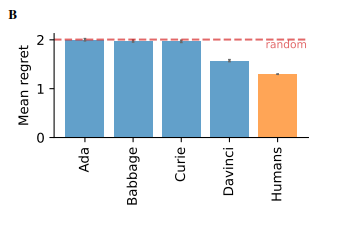
\includegraphics{img/chatgpt-engines-mean-regret.png}
		\caption{Afbeelding van \textcite{Binz2023}. Dit toont de \textit{mean regret} aan tussen de vier engines en de menselijke antwoorden.}
	\end{center}
\end{figure}

\subsubsection{Tools met GPT-3}

De mogelijkheden van OpenAI's ChatGPT en GPT-3 modellen zijn nog volop in ontwikkeling, maar er zijn al enkele vergelijkende onderzoeken uitgevoerd. Uit het experiment van \textcite{Goyal2022} blijkt dat \textit{zero-shot} samenvattingen met GPT-3 beter presteren dan \textit{fine-tuned} modellen. Daarnaast haalt \textcite{Mottesi2023} verschillende tools aan die gebruik maken van de GPT-3 API, waaronder Jasper AI en ChatSonic. Ook voor het onderwijs zijn er mogelijkheden, zoals de hoge toegankelijkheid en granulaire personalisatie van het GPT-3 model \autocite{Roose2023, Garg2022}. Echter, GPT-3 is niet geschikt voor alle taken, zoals sentimentanalyse en -classificatie, waarvoor een kleinschaliger taalmodel beter presteert \autocite{Li2022}. Bovendien is er aandacht voor de ecologische effecten van de grote omvang van deze modellen, waarvoor alternatieve oplossingen zoals het gebruik van Cloud-infrastructuur en geschikte model finetuning worden voorgesteld \autocite{Strubell2019, Simon2021}.

% Onderzoek naar OpenAI's ChatGPT en GPT-3 modellen bevindt zich in een vrij vroeg stadium, al zijn er wel enkele vergelijkende onderzoeken die de kracht en zwaktes van deze technologieën aantonen. Het experiment van \textcite{Goyal2022} achterhaalt het gebruik van \textit{zero-shot} samenvattingen buiten generieke samenvattingen. Het onderzoek staat stil bij de impact van prompt-gebaseerde modellen voor het automatisch samenvatten van nieuwsartikelen. Daarnaast maakte het onderzoek gebruik van text-davinci-002 als case study. Uit het experiment besluiten de onderzoekers dat \textit{zero-shot} samenvattingen met GPT-3 beter presteren dan \textit{fine-tuned} modellen, en dat bestaande automatische metrieken zoals BLEU, ROUGE en BERTScore niet geschikt zijn om \textit{zero-shot} samenvattingen te beoordelen. Verder blijkt dat zero-shot samenvattingen meer coherentie en relevantie hebben voor trefwoord-gebaseerde samenvattingen, terwijl aspect-gebaseerde samenvattingen nog vaak blijven te falen.

% \textcite{Mottesi2023} haalt lees- en schrijftools aan die gebruik maken van de GPT-3 API. Jasper AI is een chatbot bestemd voor customer support en een virtueel assistent voor e-commerce. ChatSonic is een tool gericht om social media posts of nieuwsartikelen te generere op basis van een kernzin of kernwoord. Verschillende artikels vermelden de mogelijkheden voor het gebruik van GPT-3 en ChatGPT in het onderwijs. \textcite{Roose2023} haalt zo de hoge toegankelijkheid, engagement bij scholieren en granulaire personalisatie aan dat het GPT-3 model toe in staat is. \textcite{Garg2022} ziet in GPT-3 en ChatGPT een portaalfunctie, om scholieren te helpen bij het opzoeken van nieuwe informatie tijdens de les en bij het instuderen.

% \textcite{Li2022} benadrukt dat GPT-3 voor simpele taken \textit{overkill} is. Taken buiten het genereren van teksten, zoals sentimentanalyse en -classificatie, worden beter met een kleinschaliger taalmodel, zoals BERT en verwante modellen, uitgevoerd. Deze keuze beïnvloedt het budget, want GPT-3 is een API waar per token wordt betaald, terwijl BERT gratis en open-source is. \textcite{Strubell2019, Simon2021} halen de ecologische effecten aan van ontwikkelaars die te snel voor deze modellen grijpen. Er is een bewezen effect kleinere modellen, gebruik van Cloud-infrastructuur en ten slotte een geschikte model finetuning bijdragen tot efficiëntere alsook minder klimaatbelastende effect.

\subsubsection{Vergelijking met andere taalmodellen}

De architectuur tussen GPT-3 en BERT is volgens \textcite{Mottesi2023} het meest opvallende verschil. GPT-3 is een autoregressief model en houdt daarmee enkel rekening met de linkercontext bij het voorspellen of genereren van tekst. BERT daarentegen is bidirectioneel en neemt zowel de linker- als de rechtercontext in overweging. De bidirectionele werking is geschikt voor sentimentanalyse waarbij begrip van de volledige zincontext noodzakelijk is. GPT-3 heeft toegang tot meer informatie (45TB) dan BERT (3TB), wat het een voordeel kan geven bij het samenvatten of het vertalen. Ten slotte zijn er ook verschillen in grootte. Hoewel beide modellen erg groot zijn, GPT-3 is aanzienlijk groter dan de voorganger vanwege de uitgebreide trainingsdatasetgrootte \autocite{Brown2020}.

LLaMa of Large Language Model Meta AI is een generatief taalmodel met potentieel dat sterker is dan GPT-3 en soortgelijke modellen, terwijl het van tien keer minder parameters gebruik maakt, maar is nog niet beschikbaar als online webtoepassing of API \autocite{Hern2023, Touvron2023}.


\begin{figure}[H]
	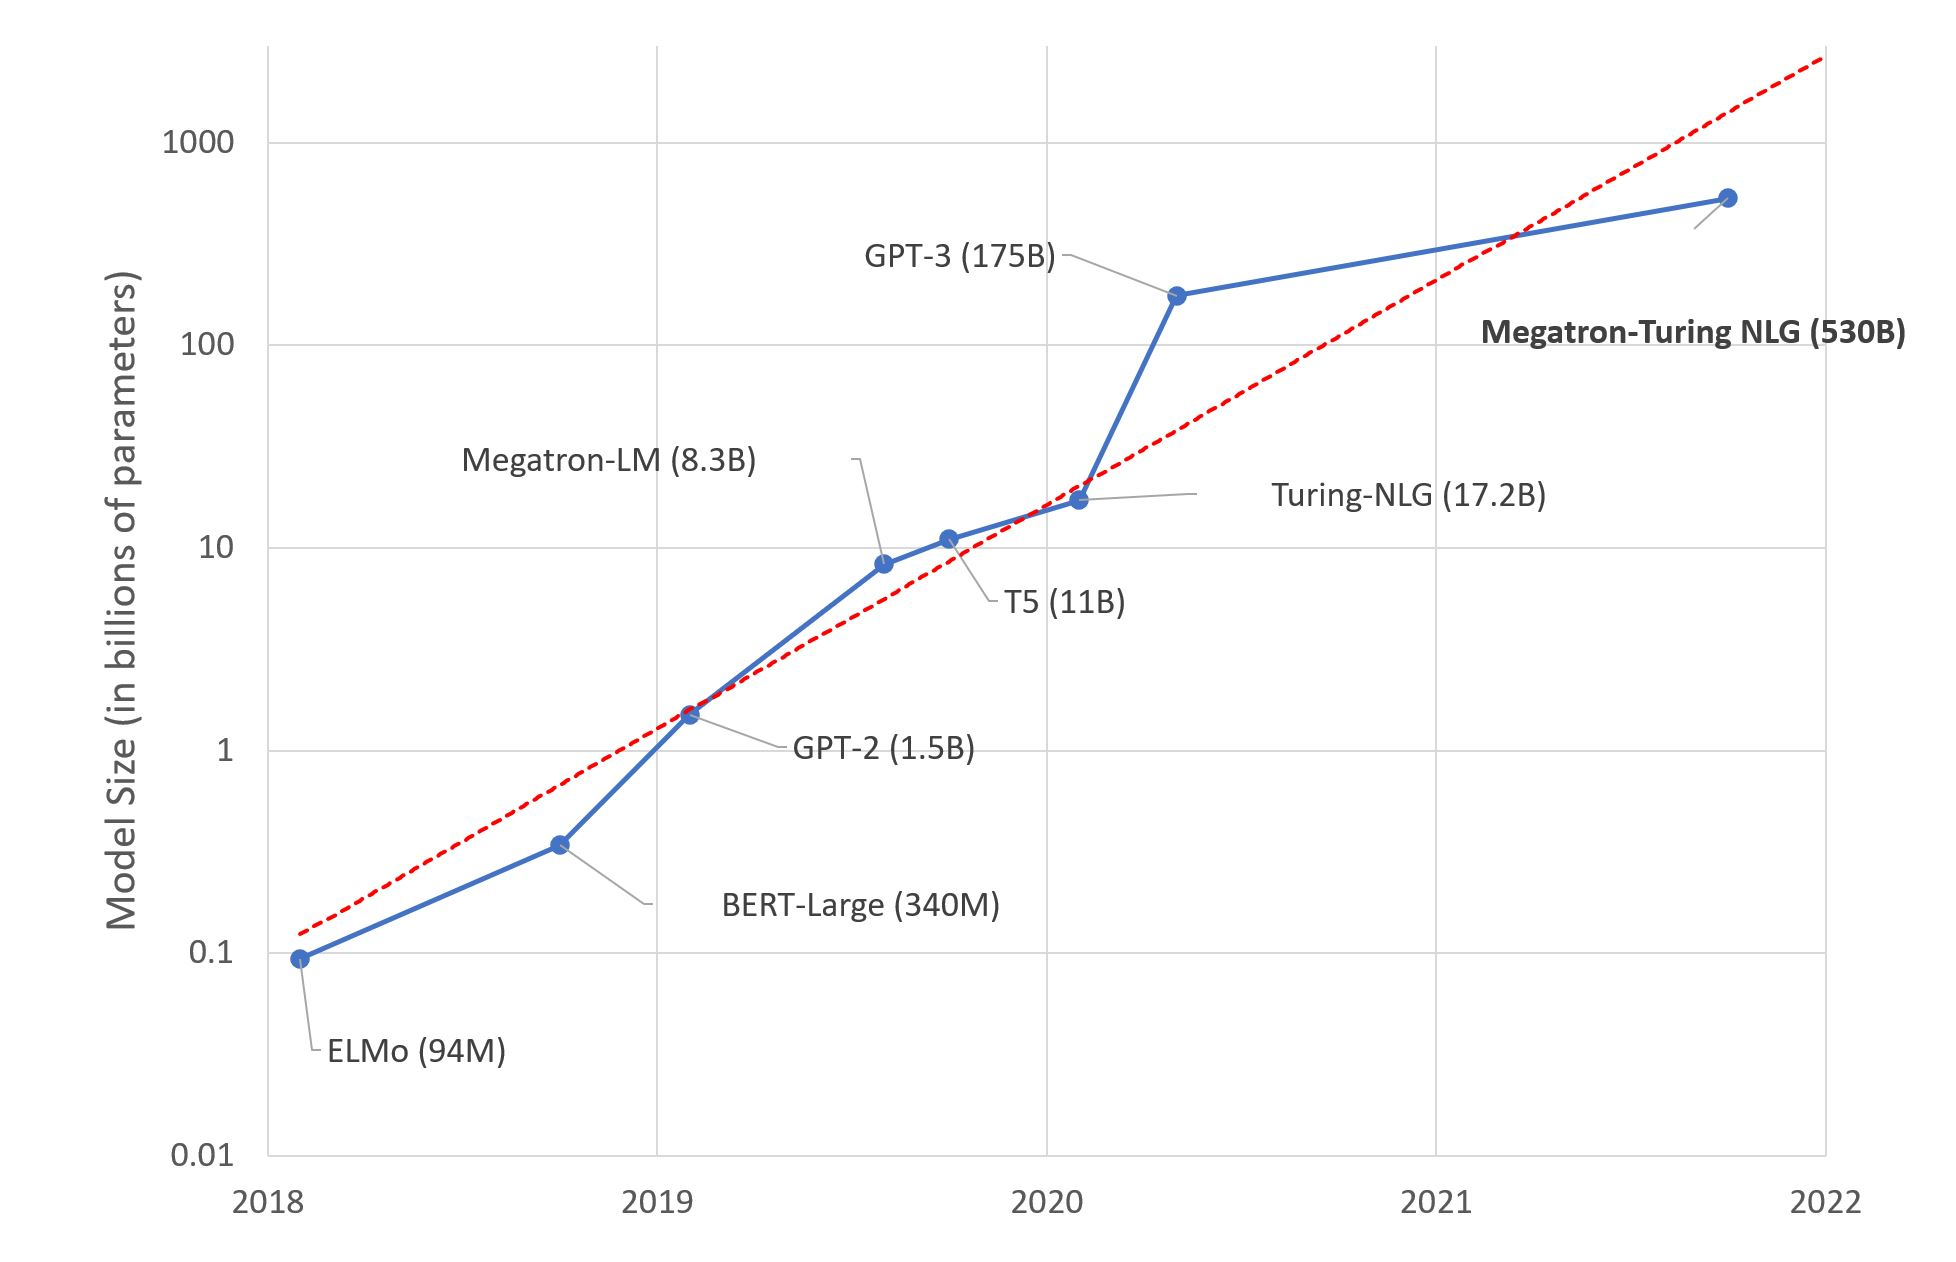
\includegraphics{img/graph-language-models.png}
	\caption{Afbeelding van \textcite{Simon2021}. De evolutie van pre-trained taalmodellen wordt hier weergegeven tot eind 2022. De performantie van de modellen ten opzichte van de grootte volgt een lineaire functie.}
\end{figure}

\subsubsection{GPT-3 finetuning}

\begin{tabular}{|c|p{7cm}|p{5cm}|}
	\hline
	Parameter & Omschrijving & Mogelijke waarden \\
	\hline
	model & Het GPT-3 model om te gebruiken & davinci, curie, babbage, ada, text-davinci-002, text-curie-001, text-babbage-001, text-ada-001, davinci-codex \\
	\hline
	temperature & De gulzigheid van een generatief model. Een lagere waarde zal conservatieve en voorspelbare tekst teruggeven. Hogere waarden zullen meer gevarieerde en onverwachtse tekst teruggeven, wat beter werkt bij creatieve toepassingen. & Een kommagetal tussen 0 en 1. \\
	\hline
	max\_tokens & Het maximaal aantal tokens (woorden of subwoorden) dat het generatief model kan teruggeven. & Een getal tussen 1 and 2048. \\
	\hline
	top\_p & Vergelijkbaar met temperature, maar deze waarde onderhoudt de probability distribution voor common tokens. Hoe lager de waarde, hoe waarschijnlijker de woordenschat dat het model zal overwegen bij het genereren van tekst. Een hoge waarde is toepasselijker wanneer een toepassing gericht is op nauwkeurigheid en correctheid. & Een kommagetal tussen 0 en 1. \\
	\hline
	stop & Een tekstwaarde (woord/symbool) tot waar het model zal genereren. When the model generates a string that matches any of the specified strings, it stops generating text. & Een lijst van string-waarden, of een enkele string. \\
	\hline
	presence\_penalty & Factor die bepaalt hoe regelmatig woorden voorkomen. & Een kommagetal tussen 0 en 1 \\
	\hline
\end{tabular}

\subsection{Bing AI}

Microsoft en OpenAI werken nauw samen. Zo maakt het conversationele taalmodel van Bing ook gebruik van GPT-3. Deze chatbot bouwt verder en biedt zo verwijzingen en referenties aan naar andere websites. Deze verwijzingen zijn volgens mogelijk door de Prometheus-technologie van Microsoft \autocite{Ribas2023}.

Prometheus is een eigen technologie die door Bing is ontwikkeld. Het AI-model is volgens \textcite{Ribas2023} de eerste van zijn soort die de Bing-index-, ranking- en antwoordresultaten combineert met het redeneervermogen van OpenAI’s GPT-modellen. Prometheus maakt gebruik van de kracht van Bing en GPT om iteratief via een component genaamd \textit{Bing Orchestrator} een set interne queries te genereren met als doel binnen gegeven gesprekscontext een nauwkeurig antwoord op gebruikersqueries te bieden \autocite{Ribas2023}.

\begin{figure}[H]
	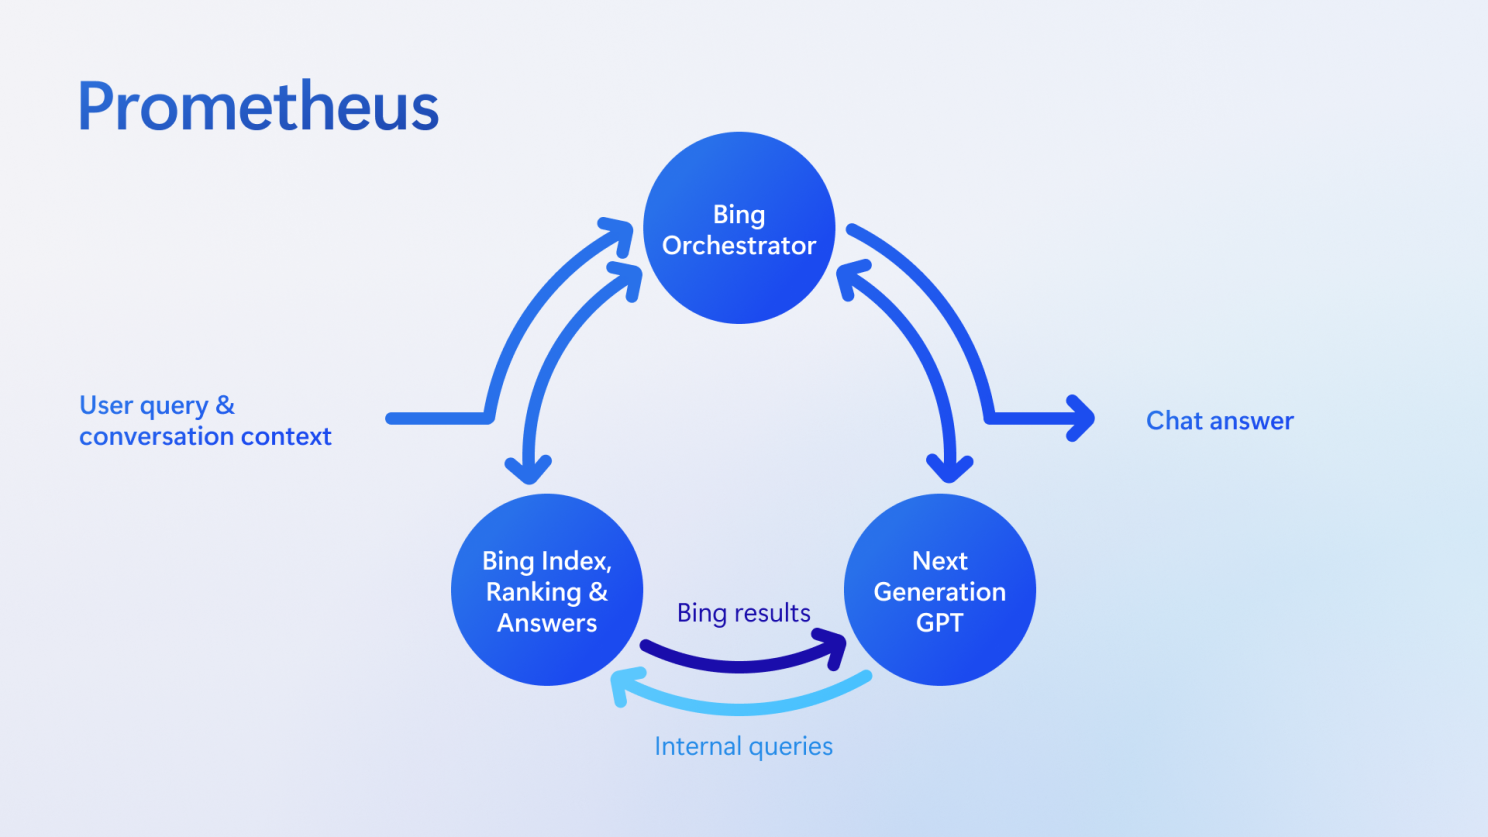
\includegraphics[width=6cm]{img/bing-ai-prometheus.png}
	\caption{Afbeelding van \textcite{Ribas2023}.}
\end{figure}

Bing AI is nu in testfase met wachtlijst en bestaat in de vorm van een webpagina en een browserextensie voor Microsoft Edge. Onderzoek naar deze chatbot staat nog in de kinderschoenen en er is nood aan onderzoek naar de credibiliteit en correctheid van de verwijzingen. Deze chatbot gebruikt een combinatie van extraherende en abstraherende samenvattingen. In tegenstelling tot GPT-3 is er geen officiële API beschikbaar. Daarnaast is de limiet ook lager met 2000 tokens per bericht tijdens een conversatie. 

\begin{figure}[H]
	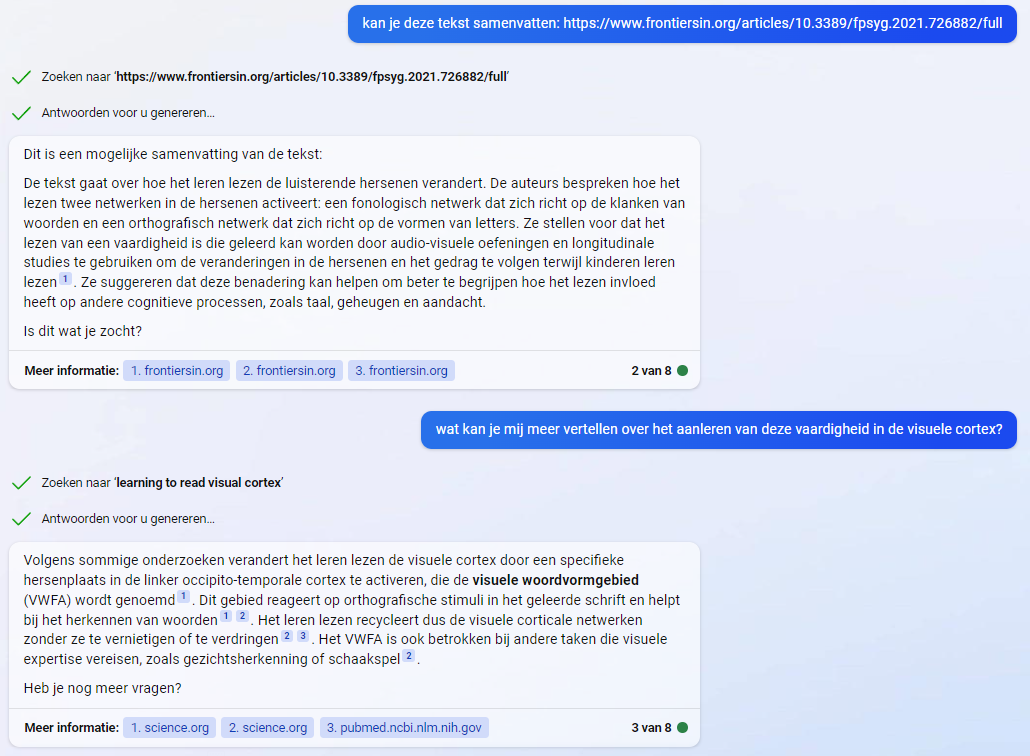
\includegraphics{img/bing-ai-chatbot-example.png}
	\caption{In deze afbeelding wordt er een online wetenschappelijk artikel meegegeven. Er wordt geen titel of onderwerp meegegeven, maar de Bing AI chatbot is in staat om een abstraherende samenvatting te maken van het artikel. Daarna geeft de chatbot verder uitleg over een bepaald onderwerp en geeft het extra referenties mee.}
\end{figure}

Het bedrijf DuckDuckGo dat instaat voor de gelijknamige zoekmachine probeert een gelijkaardig initiatief. Met \textit{DuckAssist} biedt de onderneming een eigen AI-oplossing aan om een algemene doelgroep te ondersteunen bij het opzoeken van (nieuwe) informatie. Zij halen informatie direct uit enkel Wikipedia pagina's \autocite{Weinberg2023}. Daarnaast maakt dit DuckAssist ook gebruik van het GPT-3 model. Nadelig heeft deze toepassing voorlopig beschikking tot een kleinere zoekruimte dan Bing AI, wat gebruik maakt van meer sites inclusief onderzoekssites zoals ResearchGate \autocite{Mcauliffe2023}. Deze beperkte zoekruimte reduceert de kans op incorrecte of foutieve informatie volgens \textcite{Weinberg2023}, al is dit eerder een intuïtie van het bedrijf.


\subsection{Huggingface en taalmodellen via API}

In recente literatuur is Huggingface beschreven als een platform of portaalsite voor het delen van ML-modellen en datasets. De bibliotheek biedt een scala aan API's en tools die gemakkelijk te downloaden en trainen zijn voor pretrained modellen voor prevalente NLP-taken, zoals tekstclassificatie, taalmodellering en samenvatting. Deze modellen kunnen worden gefinetuned op specifieke datasets, waardoor ontwikkelaars snel modellen kunnen bouwen en inzetten voor vereenvoudigings- en samenvattingstaken. Voor wetenschappelijke documenten en artikelen bestaan er enkel modellen en datasets: \footnote{https://huggingface.co/sambydlo/bart-large-scientific-lay-summarisation}, \footnote{https://huggingface.co/haining/scientific\_abstract\_simplification}

\subsection{Conclusie}

Experten halen het GPT-3 model en ChatGPT aan als de toekomst voor gepersonaliseerde en adaptieve uitleg aan scholieren. Bing AI biedt een extra dat revolutionair kan zijn bij het opzoeken van uitleg voor zoektermen, zonder het verlies aan bronvermelding. Huidige toepassingen staan mogelijks in een spreekwoordelijke schaduw eenmaal leessoftware voor scholieren met dyslexie worden ontwikkeld met AI. De mogelijkheden van GPT-3 zijn eindeloos en toepassingen die hiervan gebruik maken, kunnen in het onderwijs ingezet worden als ondersteunende software.

\section{Conclusie}

De noden van scholieren met fonologische dyslexie in de derde graad van het middelbaar gaan verder dan gewoon moeizaam lezen.  Het ontcijferen en automatiseren van woordeherkenning gebeurt langzaam. Er zijn bewezen voordelen van manuele tekstvereenvoudiging en adaptieve visuele weergaven op kinderen en jongeren met dyslexie. De leesbaarheid van wetenschappelijke artikelen bevindt zich in een neergaande trend. Het formaat, gebruik van vakjargon en ingewikkelde woordenschat en ten slotte de moeizame syntax en zinsbouw sluiten een algemene doelgroep uit bij het lezen van wetenschappelijke artikelen. Enkel wetenschappelijk geletterden zijn in staat om deze artikelen te lezen. Het uniforme formaat van een wetenschappelijk artikel biedt kansen aan voor een geautomatiseerde aanpak tot het vereenvoudigen van een tekst.

Experten halen meerdere bewezen tactieken aan om teksten automatisch te vereenvoudigen op maat voor een scholier met dyslexie. Handmatig worden teksten vereenvoudigd aan de hand van leesbaarheidsformules of intuïtie. Zinnen moeten lexicaal, syntactisch en semantisch worden vereenvoudigd. Teksten samenvatten maakt de tekst korter zonder het verlies van de kernboodschap. Voor deze vier transformaties zijn er taalmodellen beschikbaar in de vorm van API's of open-source software. Huidige software dat de overheid uitleent aan scholieren met dyslexie in het middelbaar onderwijs fungeert voornamelijk als voorleessoftware. Nieuwe en opkomende technologieën en taalmodellen zoals GPT-3 blinken uit om tekstvereenvoudiging mogelijk te maken. De ontwikkeling met LLM's is in opmars, maar ontwikkelaars moeten bewust zijn dat andere taalmodellen zoals BERT voor taken zoals semantische analyse minder rekenkracht vereisen voor eenzelfde en soms beter resultaat. 